
%===== main document class =====
%\ifdefined\slideModeHandout
\documentclass%
[%
  handout,          % avoid unnecessary overlays
  aspectratio=169,  % aspect ratio fo 16:9 
  t,                % place content at top of frames
  10pt,             % use 10pt as standard font size (default size is 11pt)
  compress,         % compress things like navigation bars...
]{beamer}
%\else
%\documentclass%
%[%
%  aspectratio=169,  % aspect ratio fo 16:9 
%  t,                % place content at top of frames
%  10pt,             % use 10pt as standard font size (default size is 11pt)
%  compress,         % compress things like navigation bars...
%]{beamer}
%\fi

\mode<presentation>
%===============tabto==============
% tabto.sty
%
% version 1.4  (Dec 2018)
%
% Tabbing to fixed positions in a paragraph.
%
% Copyright 2006,2009,2012,2013,2018 by 
% Donald Arseneau,   Vancouver, Canada (asnd@triumf.ca)
% Permission to use, distribute and modify this software is granted
% under the conditions of the LaTeX Project Public License, either 
% version 1.3 or (at your option) any later version.  The license is
% found at http://www.latex-project.org/lppl.txt, and is part of all 
% recent distributions of LaTeX.
%
% This work has the LPPL maintenance status `maintained' (by author).
%
% Two new text positioning commands are defined: \tabto and \tab.
% 
% \tabto{<length>}
% Tab to a position relative to the left margin in a paragraph (any
% indentation due to a list or \leftskip is part of the `margin' in
% this context). If the text on the line already goes past the desired
% position, the tab starts a new line and moves to the requested
% horizontal position.
%
% \tabto*{<length>}
% Similar to \tabto, except it will perform backspacing, and over-
% print previous text on the line whenever that text is already
% longer than the specified length (i.e., no linebreak is produced).
% Line-breaks are suppressed immediately after \tabto or \tabto*.
%
% The length register "\CurrentLineWidth" will report the width
% of the existing text on the line, and it may be used in the
% <length> argument (using calc.sty, for example). Also, there
% is "\TabPrevPos" which gives the "\CurrentLineWidth" from the
% previous tab command (the position where the tab command occurred,
% not where it went to), and can be used to return to that position
% if no line breaks have occurred in between, or directly below it,
% if there were line breaks.
%
% \tab
% Tab to the next tab-stop chosen from a list of tab positions, in
% the traditional style of typewriters.  A \tab will always move
% to the next tab stop (or the next line), even if it is already
% exactly at a tab stop. Thus, "\tab" at the beginning of a line,
% or "\tab\tab" elsewhere skips a position. A linebreak is permitted 
% immediately following a \tab, in case the ensuing text does not 
% fit well in the remaining space.
%
% If you do not want to skip positions, use "\tabto{\NextTabStop}"
% instead of "\tab".  This is particularly useful when you want to
% use \tab in some other command, but do not want to skip a column
% for the first item.
%
% The tab-stop positions are declared using either \TabPositions
% or \NumTabs:
%
% \TabPositions{<length>, <length>,...<length>}
% Declares the tab stops as a comma-separated list of positions 
% relative to the left margin. A tab-stop at 0pt is implicit, and 
% need not be listed.
%
% \NumTabs{<number>}
% Declares a list of <number> equally-spaced tabs, starting at the
% left margin and spanning \linewidth.  For example \NumTabs{2} 
% declares tab-stops at 0pt and 0.5\linewidth, the same as
% \TabPositions{0pt, 0.5\linewidth} or \TabPositions{0.5\linewidth}
%
% After these declarations, the list of tab positions is saved in
% \TabStopList, and the next tab position, relative to the current 
% position, is given by \NextTabStop.  You do not normally need
% to access them, but they are available.
%
% Problems:
%
% Tall objects after a tab stop may overlap the line above, rather
% than forcing a greater separation between lines.

%\ProvidesPackage{tabto}[2018/12/28 \space v 1.4 \space 
%  Another tabbing mechanism]\relax

%%%%%%%%%Code Begin

%\newdimen\CurrentLineWidth
%\newdimen\TabPrevPos
%
%\newcommand\tabto[1]{%
% \leavevmode
% \begingroup
% \def\@tempa{*}\def\@tempb{#1}%
% \ifx\@tempa\@tempb % \tab* 
%   \endgroup
%   \TTo@overlaptrue % ... set a flag and re-issue \tabto to get argument
%   \expandafter\tabto
% \else
%   \ifinner % in a \hbox, so ignore
%   \else % unrestricted horizontal mode
%     \null% \predisplaysize will tell the position of this box (must be box)
%     \parfillskip\fill
%     \everydisplay{}\everymath{}%
%     \predisplaypenalty\@M \postdisplaypenalty\@M
%     $$% math display so we can test \predisplaysize
%      \lineskiplimit=-999pt % so we get pure \baselineskip
%      \abovedisplayskip=-\baselineskip \abovedisplayshortskip=-\baselineskip
%      \belowdisplayskip\z@skip \belowdisplayshortskip\z@skip
%      \halign{##\cr\noalign{%
%        % get the width of the line above
%        \ifdim\predisplaysize=\maxdimen %\message{Mixed R and L, so say the line is full. }%
%           \CurrentLineWidth\linewidth
%        \else
%           \ifdim\predisplaysize=-\maxdimen 
%             % \message{Not in a paragraph, so call the line empty. }%
%             \CurrentLineWidth\z@
%           \else
%             \ifnum\TTo@Direction<\z@
%               \CurrentLineWidth\linewidth \advance\CurrentLineWidth\predisplaysize
%             \else
%               \CurrentLineWidth\predisplaysize 
%             \fi
%             % Correct the 2em offset
%             \advance\CurrentLineWidth -2em
%             \advance\CurrentLineWidth -\displayindent
%             \advance\CurrentLineWidth -\leftskip
%        \fi\fi
%        \ifdim\CurrentLineWidth<\z@ \CurrentLineWidth\z@\fi
%        % Enshrine the tab-to position; #1 might reference \CurrentLineWidth
%        \setlength\@tempdimb{#1}% allow calc.sty
%        %\message{*** Tab to \the\@tempdimb, previous width is \the\CurrentLineWidth. ***}%
%        % Save width for possible return use
%        \global\TabPrevPos\CurrentLineWidth
%        % Build the action to perform
%        \protected@xdef\TTo@action{%
%           \vrule\@width\z@\@depth\the\prevdepth
%           \ifdim\CurrentLineWidth>\@tempdimb
%              \ifTTo@overlap\else
%                 \protect\newline \protect\null
%           \fi\fi
%           \protect\nobreak
%           \protect\hskip\the\@tempdimb\relax
%        }%
%        %\message{\string\TTo@action: \meaning \TTo@action. }%
%        % get back to the baseline, regardless of its depth.
%        \vskip-\prevdepth
%        \prevdepth-99\p@
%        \vskip\prevdepth
%      }}%
%      $$
%     % Don't count the display as lines in the paragraph
%     \count@\prevgraf \advance\count@-4 \prevgraf\count@
%     \TTo@action
%     %%   \penalty\@m % to allow a penalized line break
%   \fi
%   \endgroup
%   \TTo@overlapfalse
%   \ignorespaces
% \fi
%}
%
%% \tab -- to the next position
%% \hskip so \tab\tab moves two positions
%% Allow a (penalized but flexible) line-break right after the tab.
%%
%\newcommand\tab{\leavevmode\hskip2sp\tabto{\NextTabStop}%
%  \nobreak\hskip\z@\@plus 30\p@\penalty4000\hskip\z@\@plus-30\p@\relax}
%
%
%% Expandable macro to select the next tab position from the list
%
%\newcommand\NextTabStop{%
%  \expandafter \TTo@nexttabstop \TabStopList,\maxdimen,>%
%}
%
%\def\TTo@nexttabstop #1,{%
%    \ifdim#1<\CurrentLineWidth
%      \expandafter\TTo@nexttabstop
%    \else
%      \ifdim#1<0.9999\linewidth#1\else\z@\fi
%      \expandafter\strip@prefix
%    \fi
%}
%\def\TTo@foundtabstop#1>{}
%
%\newcommand\TabPositions[1]{\def\TabStopList{\z@,#1}}
%
%\newcommand\NumTabs[1]{%
%   \def\TabStopList{}%
%   \@tempdimb\linewidth 
%   \divide\@tempdimb by#1\relax
%   \advance\@tempdimb 1sp % counteract rounding-down by \divide
%   \CurrentLineWidth\z@
%   \@whiledim\CurrentLineWidth<\linewidth\do {%
%     \edef\TabStopList{\TabStopList\the\CurrentLineWidth,}%
%     \advance\CurrentLineWidth\@tempdimb
%   }%
%   \edef\TabStopList{\TabStopList\linewidth}%
%}
%
% %default setting of tab positions:
%\TabPositions{\parindent,.5\linewidth}
%
%%\newif\ifTTo@overlap \TTo@overlapfalse
%
%%\@ifundefined{predisplaydirection}{
%% \let\TTo@Direction\predisplaysize
%% \let\predisplaydirection\@undefined
%%}{
%% \let\TTo@Direction\predisplaydirection
%%}
%
%

% ===== include packages =====
\usepackage{lmodern}
\usepackage[utf8]{inputenc}      % Unicode UTF-8 encoding support
\usepackage[T2A,T1]{fontenc}         % T1 font encoding
\usepackage{etoolbox}            % Programming tools (used for \insertpartstartframe, \insertpartendframe)
\usepackage{ifthen}              % Simple conditional statements
\usepackage{amsmath}             % AMS math package
\usepackage{amssymb}             % Extended collection of math symbols
\usepackage{mathtools}           % More math stuff
\usepackage{nicefrac}            % Nice fractions
\usepackage{xcolor}              % Driver independent colors
\usepackage{colortbl}            % rowcolor for tables
\usepackage{array}               % tables and arrays with extended features (e.g., overlays)
\usepackage{makecell}            % Simple formatting of single table cells
\usepackage{multirow}            % Multi-rows in tabular environments
\usepackage{booktabs}            % More flexible lines for tabular environments
\usepackage{tabto}               % Easy way of specifying tabulators
\usepackage{adjustbox}           % Macros for adjusting boxed content (used in defining \fitbox)
\usepackage{relsize}             % Relative font sizes (\larger=\relsize{1}, \smaller=\relsize{-1})
\usepackage{graphicx}            % Inserting pictures
\usepackage{hyperref}            % Cross referencing
%\usepackage{media9}              % Include media objects
%\usepackage{animate}             % Animations
\usepackage{tikz}                % TikZ library for drawing
\usepackage{pgfplots}            % Plots
\usepackage{import}              % including stuff with relative paths
%\usepackage{listings}            % source code inclusion

%===== TikZ libraries =====
\usetikzlibrary{shapes}          % Additional shapes: Ellipse
\usetikzlibrary{shapes.symbols}  % Additional shapes: Symbols (e.g., "cloud")
\usetikzlibrary{shapes.arrows}   % Additional shapes: Arrows (e.g., "single arrow")
\usetikzlibrary{arrows}          % Arrow tips
\usetikzlibrary{arrows.meta}     % Adjustable arrow heads
\usetikzlibrary{positioning}     % Relative positioning of nodes

%===== pgfsetting =====
\pgfplotsset{compat=newest}      % Use newest version of pgf
\usepgfplotslibrary{fillbetween} % filling between curves

%===== nice tables =====
\setlength{\heavyrulewidth}{0.08em}
\setlength{\lightrulewidth}{0.08em}
\setlength{\cmidrulewidth}{0.04em}
\setlength{\aboverulesep}{0.4ex}
\setlength{\belowrulesep}{0.6ex}
\newcommand{\cmidbeg}{\addlinespace[0.40ex]}
\newcommand{\cmidend}{\addlinespace[0.10ex]}

\usepackage{caption}
\usepackage{subcaption}


%%%%%%%%%%%%%%%%%%%%%%%%%%%%%%%%%%%%%%%%%%%%%%%%%%%%%%%%%%%%
%%%%%%
%%%%%%     M A I N   D O C U M E N T   S W I T C H E S     
%%%%%%
%%%%%%%%%%%%%%%%%%%%%%%%%%%%%%%%%%%%%%%%%%%%%%%%%%%%%%%%%%%%

% define command for directly using switches
\newcommand{\usetoggle}[1]{\iftoggle{#1}{true}{false}}

% define switches
\newtoggle{useNavSymbols}               % display of navigation symbols
\newtoggle{useShadows}                  % use blocks with shadows
\newtoggle{useColorBlocks}              % use colored blocks
\newtoggle{useColorBlockTitles}         % use colored block titles
\newtoggle{useInverseBlockTitles}       % use colored block title background with white text
\newtoggle{altColors}                   % use alternative color theme
\newtoggle{addExercises}                % whether exercises are used
\newtoggle{specialHeiko}                % special stuff for Heiko
\newtoggle{specialThomas}               % special stuff for Thomas

\def\slideStyleThomas{..}


\ifdefined\slideStyleThomas

  %>>>>>>>>>> parameters for Thomas >>>>>>>>>>
  \title%
      [Image and Video Coding]%
      {Image and Video Coding I:\\[0.5ex] Fundamentals}
  \author%
      [T. Wiegand, J. Pfaff, J. Rasch]%
      {Thomas Wiegand, Jonathan Pfaff, Jennifer Rasch}
  \institute%
      [TU Berlin, Fraunhofer HHI]%
      {Technische Universität Berlin, Fraunhofer Heinrich Hertz Institute, Berlin}

  \newcommand{\slideOrganization}{}

  \settoggle{useNavSymbols}        {false}
  \settoggle{useShadows}           {true}
  \settoggle{useColorBlocks}       {true}
  \settoggle{useColorBlockTitles}  {true}
  \settoggle{useInverseBlockTitles}{true}
  \settoggle{altColors}            {false}
  \settoggle{addExercises}         {false}

  \settoggle{specialHeiko}         {false}
  \settoggle{specialThomas}        {true}
  %<<<<<<<<<< parameters for Thomas <<<<<<<<<<

\else

  %>>>>>>>>>> parameters for Heiko >>>>>>>>>>
  \title%
      {Data Compression}
  \author%
      [Heiko Schwarz]%
      {Heiko Schwarz}
  \institute%
      [Freie Universität Berlin]%
      {Freie Universität Berlin\\%
      Fachbereich Mathematik und Informatik}

\ifdefined\slideModeHandout
  \settoggle{useNavSymbols}        {false}
\else
  \settoggle{useNavSymbols}        {false}
\fi
  \settoggle{useShadows}           {true}
  \settoggle{useColorBlocks}       {true}
  \settoggle{useColorBlockTitles}  {true}
  \settoggle{useInverseBlockTitles}{true}
  \settoggle{altColors}            {false}
  \settoggle{addExercises}         {true}

  \settoggle{specialHeiko}         {true}
  \settoggle{specialThomas}        {false}
  %<<<<<<<<<< parameters for Heiko <<<<<<<<<<

\fi % end of conditional





%%%%%%%%%%%%%%%%%%%%%%%%%%%%%%%%%%%%%%%%%%%%%%%%%
%%%%%%
%%%%%%     C U S T O M I Z E   D E S I G N
%%%%%%
%%%%%%%%%%%%%%%%%%%%%%%%%%%%%%%%%%%%%%%%%%%%%%%%%

%===== spacing for lists and paragraphs (modified copy from beamerbaselocalstructure.sty) =====
\makeatletter
\setlength  \parskip         {2ex}
\setlength  \leftmargini     {2em}
\setlength  \leftmarginii    {2em}
\setlength  \leftmarginiii   {2em}
\setlength  \labelsep        {.5em}
\setlength  \labelwidth      {\leftmargini}
\addtolength\labelwidth      {-\labelsep}
\def\@listi  {\leftmargin\leftmargini
              \partopsep  \parskip
              \parskip    0.0\p@
              \parsep     0.0\p@
              \topsep     3.0\p@ \@plus1.0\p@ \@minus2.0\p@
              \itemsep    3.0\p@ \@plus1.0\p@ \@minus2.0\p@}
\let\@listI\@listi
\def\@listii {\leftmargin\leftmarginii
              \parsep     0.0\p@
              \topsep     3.0\p@ \@plus1.0\p@ \@minus2.0\p@
              \itemsep    3.0\p@ \@plus1.0\p@ \@minus2.0\p@}
\def\@listiii{\leftmargin\leftmarginiii
              \parsep     0.0\p@
              \topsep     3.0\p@ \@plus1.0\p@ \@minus2.0\p@
              \itemsep    3.0\p@ \@plus1.0\p@ \@minus2.0\p@}
\makeatother


%===== counter for exercises =====
\newcounter{exercise}


%===== enumerate symbols (modified copy from beamerbaseauxtemplates.sty) =====
\makeatletter

%--- define commands for changing enum style ---
\newcommand{\setenumstyledepth}[2]{% {enumdepth}{command for displaying counter}
  \ifthenelse{\equal{#1}{1}}%
     {\renewcommand*{\theenumi}{#2{enumi}}}%
     {\ifthenelse{\equal{#1}{2}}%
        {\renewcommand*{\theenumii}{#2{enumii}}}%
        {\renewcommand*{\theenumiii}{#2{enumiii}}}%
     }%
}
% Note: For the following command you can also use your own styles.
%       For example, a style "A." in a smaller font can be defined by
%         \newcommand{\AlphaDot}[1]{{\smaller\smaller\Alph{#1}.}}
\newcommand{\enumStyle}[1]{\setenumstyledepth{\the\@enumdepth}{#1}}
\newcommand{\enumStylesDefault}[3]{%
  \setenumstyledepth{1}{#1}%
  \setenumstyledepth{2}{#2}%
  \setenumstyledepth{3}{#3}%
}

%--- define commands for putting enum symbols ---
\newcommand{\putenumsquare}[1]{%
  \smaller%
  \usebeamercolor[bg]{\beameritemnestingprefix item projected}%
  \begin{pgfpicture}{-1ex}{-0.25ex}{1.1ex}{2.0ex}%
    \pgfpathrectangle{\pgfpoint{-1.2ex}{-0.6ex}}{\pgfpoint{2.4ex}{2.4ex}}%
    \pgfusepath{fill}%
    \pgftext[base,y=-0.15ex]{\color{fg}#1}%
  \end{pgfpicture}%
}
\newcommand{\putenumcircle}[1]{%
  \smaller%
  \usebeamercolor[bg]{\beameritemnestingprefix item projected}%
  \begin{pgfpicture}{-1ex}{-0.25ex}{1.1ex}{2.0ex}%
    \pgfpathcircle{\pgfpoint{0pt}{.6ex}}{1.3ex}%
    \pgfusepath{fill}%
    \pgftext[base,y=-0.15ex]{\color{fg}#1}%
  \end{pgfpicture}%
}
\newcommand{\putenumblank}[1]{%
  \smaller%
  \begin{pgfpicture}{-1ex}{-0.25ex}{1.1ex}{2.0ex}%
    \pgfpathrectangle{\pgfpoint{-1.2ex}{-0.6ex}}{\pgfpoint{2.4ex}{2.4ex}}%
    \pgftext[base,y=-0.15ex]{#1}%
  \end{pgfpicture}%
}
\newcommand{\putenumbracket}[1]{%
  \smaller%
  \begin{pgfpicture}{-1ex}{-0.25ex}{1.1ex}{2.0ex}%
    \pgfpathrectangle{\pgfpoint{-1.2ex}{-0.6ex}}{\pgfpoint{2.4ex}{2.4ex}}%
    \pgftext[base,y=-0.15ex]{$\boldsymbol{\langle}$#1$\boldsymbol{\rangle}$}%
  \end{pgfpicture}%
}
\newcommand{\putenumautoi}[1]{\putenumcircle{#1}}
\newcommand{\putenumautoii}[1]{\putenumcircle{#1}}
\newcommand{\putenumautoiii}[1]{\putenumcircle{#1}}
\newcommand{\putenumauto}[1]{%
  \ifthenelse{\equal{\the\@itemdepth}{1}}%
     {\putenumautoi{#1}}%
     {\ifthenelse{\equal{\the\@itemdepth}{2}}%
        {\putenumautoii{#1}}%
        {\putenumautoiii{#1}}%
     }%
}

%--- define beamer enum templates [square][circle][blank][bracket][auto] ---
\expandafter\let\csname beamer@@tmpop@enumerate item@square\endcsname\relax
\expandafter\let\csname beamer@@tmpop@enumerate subitem@square\endcsname\relax
\expandafter\let\csname beamer@@tmpop@enumerate subsubitem@square\endcsname\relax
\expandafter\let\csname beamer@@tmpop@enumerate mini template@square\endcsname\relax

\expandafter\let\csname beamer@@tmpop@enumerate item@circle\endcsname\relax
\expandafter\let\csname beamer@@tmpop@enumerate subitem@circle\endcsname\relax
\expandafter\let\csname beamer@@tmpop@enumerate subsubitem@circle\endcsname\relax
\expandafter\let\csname beamer@@tmpop@enumerate mini template@circle\endcsname\relax

\defbeamertemplate{enumerate item}{square}{\putenumsquare{\insertenumlabel}}
\defbeamertemplate{enumerate subitem}{square}{\putenumsquare{\insertsubenumlabel}}
\defbeamertemplate{enumerate subsubitem}{square}{\putenumsquare{\insertsubsubenumlabel}}
\defbeamertemplate{enumerate mini template}{square}{\putenumsquare{\insertenumlabel}}

\defbeamertemplate{enumerate item}{circle}{\putenumcircle{\insertenumlabel}}
\defbeamertemplate{enumerate subitem}{circle}{\putenumcircle{\insertsubenumlabel}}
\defbeamertemplate{enumerate subsubitem}{circle}{\putenumcircle{\insertsubsubenumlabel}}
\defbeamertemplate{enumerate mini template}{circle}{\putenumcircle{\insertenumlabel}}

\defbeamertemplate{enumerate item}{blank}{\putenumblank{\insertenumlabel}}
\defbeamertemplate{enumerate subitem}{blank}{\putenumblank{\insertsubenumlabel}}
\defbeamertemplate{enumerate subsubitem}{blank}{\putenumblank{\insertsubsubenumlabel}}
\defbeamertemplate{enumerate mini template}{blank}{\putenumblank{\insertenumlabel}}

\defbeamertemplate{enumerate item}{bracket}{\putenumbracket{\insertenumlabel}}
\defbeamertemplate{enumerate subitem}{bracket}{\putenumbracket{\insertsubenumlabel}}
\defbeamertemplate{enumerate subsubitem}{bracket}{\putenumbracket{\insertsubsubenumlabel}}
\defbeamertemplate{enumerate mini template}{bracket}{\putenumbracket{\insertenumlabel}}

\defbeamertemplate{enumerate item}{auto}{\putenumauto{\insertenumlabel}}
\defbeamertemplate{enumerate subitem}{auto}{\putenumauto{\insertsubenumlabel}}
\defbeamertemplate{enumerate subsubitem}{auto}{\putenumauto{\insertsubsubenumlabel}}
\defbeamertemplate{enumerate mini template}{auto}{\putenumauto{\insertenumlabel}}

%--- define commands for easily changing enum modes ---
% The outcommented simple version has a problem with enum nested in itemize (wrong level)
%   \newcommand{\enumMode}[1]{\setbeamertemplate{enumerate \beameritemnestingprefix item}[#1]} 
\newcommand{\enumMode}[1]{%
  \ifthenelse{\equal{\the\@enumdepth}{1}}%
     {\setbeamertemplate{enumerate item}[#1]}%
     {\ifthenelse{\equal{\the\@enumdepth}{2}}%
        {\setbeamertemplate{enumerate subitem}[#1]}%
        {\setbeamertemplate{enumerate subsubitem}[#1]}%
     }%
}
\newcommand{\enumAutoDefault}[3]{%
  \renewcommand*{\putenumautoi}[1]{\csname putenum#1\endcsname{##1}}%
  \renewcommand*{\putenumautoii}[1]{\csname putenum#2\endcsname{##1}}%
  \renewcommand*{\putenumautoiii}[1]{\csname putenum#3\endcsname{##1}}%
}

\makeatother



%===== itemize symbols (modified copy from beamerbaseauxtemplates.sty) =====
\makeatletter

%--- new item symbols ---
\newcommand{\isquare}{%
  \begin{pgfpicture}%
    \pgfpathrectangle{\pgfpointorigin}{\pgfpoint{1.0ex}{1.0ex}}%
    \pgfusepath{fill}%
    \pgfsetbaseline{-0.2ex}%
  \end{pgfpicture}%
}
\newcommand{\icircle}{%
  \begin{pgfpicture}%
    \pgfpathcircle{\pgfpoint{0pt}{.5ex}}{0.5ex}%
    \pgfusepath{fill}%
    \pgfsetbaseline{-0.2ex}%
  \end{pgfpicture}%
}
\newcommand{\itriangle}{%
  \begin{pgfpicture}%
    \pgfpathmoveto{\pgfpointorigin}
    \pgfpathlineto{\pgfpoint{0.0ex}{1.0ex}}%
    \pgfpathlineto{\pgfpoint{1.0ex}{0.5ex}}%
    \pgfusepath{fill}%
    \pgfsetbaseline{-0.2ex}%
  \end{pgfpicture}%
}
\newcommand{\idash}{%
  \begin{pgfpicture}%
    \pgfpathrectangle{\pgfpoint{0.0ex}{0.4ex}}{\pgfpoint{1.0ex}{0.2ex}}%
    \pgfusepath{fill}%
    \pgfsetbaseline{-0.2ex}%
  \end{pgfpicture}%
}
\newcommand{\iarrow}{%
  \begin{pgfpicture}%
    \pgfpathmoveto{\pgfpointorigin}
    \pgfpathlineto{\pgfpoint{-0.80ex}{ 0.75ex}}%    (-hl)( ht)  % tl =      total length
    \pgfpathlineto{\pgfpoint{-0.80ex}{ 0.25ex}}%    (-hl)( tt)  % tt = half total thickness
    \pgfpathlineto{\pgfpoint{-2.00ex}{ 0.25ex}}%    (-tl)( tt)  % hl =      head length
    \pgfpathlineto{\pgfpoint{-2.00ex}{-0.25ex}}%    (-tl)(-tt)  % ht = half head thickness
    \pgfpathlineto{\pgfpoint{-0.80ex}{-0.25ex}}%    (-hl)(-tt)
    \pgfpathlineto{\pgfpoint{-0.80ex}{-0.75ex}}%    (-hl)(-ht)
    \pgfusepath{fill}%
  \end{pgfpicture}%
}
\newcommand{\idarrow}{%
  \begin{pgfpicture}%
    \pgfpathmoveto{\pgfpointorigin}
    \pgfpathlineto{\pgfpoint{-0.80ex}{ 0.75ex}}%    (-hl)( ht)  % tl =      total length
    \pgfpathlineto{\pgfpoint{-0.80ex}{ 0.25ex}}%    (-hl)( tt)  % tt = half total thickness
    \pgfpathlineto{\pgfpoint{-2.00ex}{ 0.25ex}}%    (-tl)( tt)  % hl =      head length
    \pgfpathlineto{\pgfpoint{-2.00ex}{ 0.75ex}}%
    \pgfpathlineto{\pgfpoint{-2.80ex}{ 0.00ex}}%
    \pgfpathlineto{\pgfpoint{-2.00ex}{-0.75ex}}%
    \pgfpathlineto{\pgfpoint{-2.00ex}{-0.25ex}}%    (-tl)(-tt)  % ht = half head thickness
    \pgfpathlineto{\pgfpoint{-0.80ex}{-0.25ex}}%    (-hl)(-tt)
    \pgfpathlineto{\pgfpoint{-0.80ex}{-0.75ex}}%    (-hl)(-ht)
    \pgfusepath{fill}%
  \end{pgfpicture}%
}

%--- define beamer item templates [square][circle][triangle][dash][arrow] ---
\expandafter\let\csname beamer@@tmpop@itemize item@square\endcsname\relax
\expandafter\let\csname beamer@@tmpop@itemize subitem@square\endcsname\relax
\expandafter\let\csname beamer@@tmpop@itemize subsubitem@square\endcsname\relax

\expandafter\let\csname beamer@@tmpop@itemize item@circle\endcsname\relax
\expandafter\let\csname beamer@@tmpop@itemize subitem@circle\endcsname\relax
\expandafter\let\csname beamer@@tmpop@itemize subsubitem@circle\endcsname\relax

\expandafter\let\csname beamer@@tmpop@itemize item@triangle\endcsname\relax
\expandafter\let\csname beamer@@tmpop@itemize subitem@triangle\endcsname\relax
\expandafter\let\csname beamer@@tmpop@itemize subsubitem@triangle\endcsname\relax

\defbeamertemplate{itemize item}{square}{\isquare}
\defbeamertemplate{itemize subitem}{square}{\isquare}
\defbeamertemplate{itemize subsubitem}{square}{\isquare}

\defbeamertemplate{itemize item}{circle}{\icircle}
\defbeamertemplate{itemize subitem}{circle}{\icircle}
\defbeamertemplate{itemize subsubitem}{circle}{\icircle}

\defbeamertemplate{itemize item}{triangle}{\itriangle}
\defbeamertemplate{itemize subitem}{triangle}{\itriangle}
\defbeamertemplate{itemize subsubitem}{triangle}{\itriangle}

\defbeamertemplate{itemize item}{dash}{\idash}
\defbeamertemplate{itemize subitem}{dash}{\idash}
\defbeamertemplate{itemize subsubitem}{dash}{\idash}

\defbeamertemplate{itemize item}{arrow}{\iarrow}
\defbeamertemplate{itemize subitem}{arrow}{\iarrow}
\defbeamertemplate{itemize subsubitem}{arrow}{\iarrow}

%--- define command for easily changing item styles ---
\newcommand{\itemMode}[1]{\setbeamertemplate{itemize \beameritemnestingprefix item}[#1]}

\makeatother



%===== commands for text highlighting  =====
% helping command
\newcommand{\setfontrm} {\fontshape{\rmdefault}\selectfont}
\newcommand{\setfontit} {\fontshape{\itdefault}\selectfont}
\newcommand{\setfontrs} {\fontseries{\mddefault}\selectfont}
\newcommand{\setfontbs} {\fontseries{\bfdefault}\selectfont}
\newcommand{\setfontrrm}{\fontseries{\mddefault}\fontshape{\rmdefault}\selectfont}
\newcommand{\setfontrit}{\fontseries{\mddefault}\fontshape{\itdefault}\selectfont}
\newcommand{\setfontbrm}{\fontseries{\bfdefault}\fontshape{\rmdefault}\selectfont}
\newcommand{\setfontbit}{\fontseries{\bfdefault}\fontshape{\itdefault}\selectfont}
% normal text attributes:
  % setting series
  \newcommand<>{\regu}  [1]{{\only#2{\setfontrs}#1}}
  \newcommand<>{\bold}  [1]{{\only#2{\setfontbs}#1}}
  % setting shape
  \newcommand<>{\norm}  [1]{{\only#2{\setfontrm}#1}}
  \newcommand<>{\ital}  [1]{{\only#2{\setfontit}#1}}
  % setting series and shape
  \newcommand<>{\rnorm} [1]{{\only#2{\setfontrrm}#1}}
  \newcommand<>{\rital} [1]{{\only#2{\setfontrit}#1}}
  \newcommand<>{\bnorm} [1]{{\only#2{\setfontbrm}#1}}
  \newcommand<>{\bital} [1]{{\only#2{\setfontbit}#1}}
% special text highlighting:
  % changing color only
\renewcommand<>{\alert} [1]{{\only#2{\usebeamercolor{alerted text}\color{fg}}#1}}
  \newcommand<>{\struc} [1]{{\only#2{\usebeamercolor{structure}\color{fg}}#1}}
  \newcommand<>{\examp} [1]{{\only#2{\usebeamercolor{example text}\color{fg}}#1}}
  % changing color and series
  \newcommand<>{\Alert} [1]{{\only#2{\setfontrs\usebeamercolor{alerted text}\color{fg}}#1}}
  \newcommand<>{\Struc} [1]{{\only#2{\setfontrs\usebeamercolor{structure}\color{fg}}#1}}
  \newcommand<>{\Examp} [1]{{\only#2{\setfontrs\usebeamercolor{example text}\color{fg}}#1}}
  \newcommand<>{\ALERT} [1]{{\only#2{\setfontbs\usebeamercolor{alerted text}\color{fg}}#1}}
  \newcommand<>{\STRUC} [1]{{\only#2{\setfontbs\usebeamercolor{structure}\color{fg}}#1}}
  \newcommand<>{\EXAMP} [1]{{\only#2{\setfontbs\usebeamercolor{example text}\color{fg}}#1}}
  % changing color and shape
  \newcommand<>{\ralert}[1]{{\only#2{\setfontrm\usebeamercolor{alerted text}\color{fg}}#1}}
  \newcommand<>{\rstruc}[1]{{\only#2{\setfontrm\usebeamercolor{structure}\color{fg}}#1}}
  \newcommand<>{\rexamp}[1]{{\only#2{\setfontrm\usebeamercolor{example text}\color{fg}}#1}}
  \newcommand<>{\ialert}[1]{{\only#2{\setfontit\usebeamercolor{alerted text}\color{fg}}#1}}
  \newcommand<>{\istruc}[1]{{\only#2{\setfontit\usebeamercolor{structure}\color{fg}}#1}}
  \newcommand<>{\iexamp}[1]{{\only#2{\setfontit\usebeamercolor{example text}\color{fg}}#1}}
  % changing color, shape, and series
  \newcommand<>{\rAlert}[1]{{\only#2{\setfontrrm\usebeamercolor{alerted text}\color{fg}}#1}}
  \newcommand<>{\rStruc}[1]{{\only#2{\setfontrrm\usebeamercolor{structure}\color{fg}}#1}}
  \newcommand<>{\rExamp}[1]{{\only#2{\setfontrrm\usebeamercolor{example text}\color{fg}}#1}}
  \newcommand<>{\rALERT}[1]{{\only#2{\setfontbrm\usebeamercolor{alerted text}\color{fg}}#1}}
  \newcommand<>{\rSTRUC}[1]{{\only#2{\setfontbrm\usebeamercolor{structure}\color{fg}}#1}}
  \newcommand<>{\rEXAMP}[1]{{\only#2{\setfontbrm\usebeamercolor{example text}\color{fg}}#1}}
  \newcommand<>{\iAlert}[1]{{\only#2{\setfontrit\usebeamercolor{alerted text}\color{fg}}#1}}
  \newcommand<>{\iStruc}[1]{{\only#2{\setfontrit\usebeamercolor{structure}\color{fg}}#1}}
  \newcommand<>{\iExamp}[1]{{\only#2{\setfontrit\usebeamercolor{example text}\color{fg}}#1}}
  \newcommand<>{\iALERT}[1]{{\only#2{\setfontbit\usebeamercolor{alerted text}\color{fg}}#1}}
  \newcommand<>{\iSTRUC}[1]{{\only#2{\setfontbit\usebeamercolor{structure}\color{fg}}#1}}
  \newcommand<>{\iEXAMP}[1]{{\only#2{\setfontbit\usebeamercolor{example text}\color{fg}}#1}}
% specials: Emphasizing and names [May want to redefine in actually used style]
\renewcommand<>{\emph}  [1]{\alert#2{#1}}
  \newcommand<>{\Emph}  [1]{\ALERT#2{#1}}
  \newcommand<>{\EMPH}  [1]{\iALERT#2{#1}}
  \newcommand  {\aname} [1]{{\rmfamily\scshape #1}}



%===== define subblock environments =====
\makeatletter
\newenvironment{nesting}{%
  \par\hspace{2\beamer@leftmargin}
  \begin{minipage}{\linewidth-\beamer@leftmargin-3.5\beamer@rightmargin}%
}{%
  \end{minipage}
}
\makeatother



%===== define hooks for accessing frame number inside part  =====
\makeatletter
\newcount\beamer@partstartframe
\beamer@partstartframe=1
\apptocmd{\beamer@part}{\addtocontents{nav}{\protect\headcommand{%
    \protect\beamer@partframes{\the\beamer@partstartframe}{\the\c@framenumber}}}}{}{}
\apptocmd{\beamer@part}{\beamer@partstartframe=\c@framenumber\advance\beamer@partstartframe by1\relax}{}{}
\AtEndDocument{\immediate\write\@auxout{\string\@writefile{nav}%
    {\noexpand\headcommand{\noexpand\beamer@partframes{\the\beamer@partstartframe}{\the\c@framenumber}}}}}{}{}
\def\beamer@startframeofpart{1}
\def\beamer@endframeofpart{1}
\def\beamer@partframes#1#2{%
    \ifnum\c@framenumber<#1%
    \else%
    \ifnum\c@framenumber>#2%
    \else%
    \gdef\beamer@startframeofpart{#1}%
    \gdef\beamer@endframeofpart{#2}%
    \fi%
    \fi%
}
\newcommand\insertpartstartframe{\beamer@startframeofpart}
\newcommand\insertpartendframe{\beamer@endframeofpart}
\makeatother
\def\inserttotalpartframenumber{%
    \pgfmathparse{(\insertpartendframe-\insertpartstartframe+1)}%
    \pgfmathprintnumber[fixed,precision=2]{\pgfmathresult}%
}
\def\insertpartframenumber{%
    \pgfmathparse{(\insertframenumber-\insertpartstartframe+1)}%
    \pgfmathprintnumber[fixed,precision=2]{\pgfmathresult}%
}



%===== define visible on macro for tikz pictures  =====
% see https://tex.stackexchange.com/questions/55806/mindmap-tikzpicture-in-beamer-reveal-step-by-step#55849
\tikzset{
  invisible/.style={opacity=0},
  visible on/.style={alt={#1{}{invisible}}},
  alt/.code args={<#1>#2#3}{%
    \alt<#1>{\pgfkeysalso{#2}}{\pgfkeysalso{#3}} % \pgfkeysalso doesn't change the path
  },
  action/.code args={<#1>#2}{%
    \action<#1>{\pgfkeysalso{#2}} % \pgfkeysalso doesn't change the path
  },
}
% see https://tex.stackexchange.com/questions/6135/how-to-make-beamer-overlays-with-tikz-node
\tikzset{onslide/.code args={<#1>#2}{% \pgfkeysalso doesn't change the path
  \only<#1>{\pgfkeysalso{#2}} %
}}
\tikzset{temporal/.code args={<#1>#2#3#4}{% \pgfkeysalso doesn't change the path
  \temporal<#1>{\pgfkeysalso{#2}}{\pgfkeysalso{#3}}{\pgfkeysalso{#4}} %
}}


%===== further helpful tikz macros =====
\newcommand{\budash}{{\tikz[baseline=0.1ex]\draw[thick](0,0)--({0.6em},0);}}
\newcommand{\nudash}{{\tikz[baseline=0.1ex]\draw[]     (0,0)--({0.6em},0);}}



%===== define a fitbox command  =====
\makeatletter
\newlength{\fitboxw}
\newlength{\fitboxh}
\newlength{\slideinnerheight}
\setlength{\slideinnerheight}{0.85\textheight} %%% could be reset later
\newcommand<>{\fitbox}[4][c]{%
  \only#5{%
    {%
      \setlength{\fitboxw}{#2}%
      \setlength{\fitboxh}{#3}%
      \parbox[#1][\fitboxh]{\fitboxw}{%
        \centering%
        \vfill%
        \adjustbox{%
          min width=\fitboxw,%
          min height=\fitboxh,%
          max width=\fitboxw,%
          max height=\fitboxh%
        }%
        {#4}%
        \vfill%
      }%
    }%
  }%
}
\newcommand<>{\hfitbox}[3][c]{%
  \only#4{%
    {%
      \setlength{\fitboxw}{#2}%
      \parbox[#1]{\fitboxw}{%
        \adjustbox{%
          min width=\fitboxw,%
          max width=\fitboxw}%
        {#3}%
      }%
    }%
  }%
}
\newcommand<>{\slidehfitbox}[1]{%
  \hfitbox#2{\textwidth}{#1}%
}
\newcommand<>{\slidefitbox}[1]{%
  \fitbox#2{\textwidth}{\slideinnerheight}{#1}%
}
\makeatother



%===== command for adding new part with part page / adding title page  =====
\newcommand{\startnewpart}[2][\usebeamercolor{background}\color{bg}\rule{1pt}{1pt}]{
  \part{#2}
  {
    \setbeamertemplate{navigation symbols}{}
    \begin{frame}[plain]
    \vfill\vfill
    {\hfill\begin{beamercolorbox}[%
       sep=8pt,dp=1ex,center,wd=0.8\textwidth,%
       rounded=true,
       shadow=\usetoggle{useShadows}%
    ]%
    {part title}
    \usebeamerfont{part title}\insertpart\par
    \end{beamercolorbox}\hfill}
    \vfill
    {\hfill{\fitbox{0.8\textwidth}{0.45\textheight}{#1}}\hfill}
    \vspace{0pt}
    \end{frame}
  }
}
\newcommand{\addtitlepage}{
  {
    \setbeamertemplate{navigation symbols}{}
    \begin{frame}[plain]
    \vspace{0.15\textheight}
    {\hfill\begin{beamercolorbox}[%
       sep=8pt,dp=1ex,center,wd=0.8\textwidth,%
       rounded=true,
       shadow=\usetoggle{useShadows}%
    ]%
    {title}
    \usebeamerfont{title}\inserttitle\par
    \end{beamercolorbox}\hfill}

    \begin{center}\large
      ~\\[3ex]
      {\insertauthor}\\[3ex]
      {\insertinstitute}
    \end{center}
    \end{frame}
  }
}







%%%%%%%%%%%%%%%%%%%%%%%%%%%%%%%%%%%%%%%%%%%
%%%%%%
%%%%%%     T E M P L A T E
%%%%%%
%%%%%%%%%%%%%%%%%%%%%%%%%%%%%%%%%%%%%%%%%%%

%===== other font size =====
\makeatletter
\newcommand\notsotiny{\@setfontsize\notsotiny\@vipt\@viipt}
\makeatother

%===== font theme =====
\usefonttheme{structurebold}
\setbeamerfont{title in head/foot}{size=\tiny}
\setbeamerfont{author in head/foot}{size=\tiny}
\setbeamerfont{date in head/foot}{size=\tiny}
\setbeamerfont*{frametitle}{family=\sffamily,series=\bfseries,shape=\upshape,size=\large}


%===== color theme (based on color theme "beaver") =====
%>>> define colors (see http://latexcolor.com/ for a good visual comparison)
% reds
\definecolor{bostonuniversityred}     {rgb}{0.80, 0.00, 0.00} % used in beaver
\definecolor{cornellred}              {rgb}{0.70, 0.11, 0.11}
\definecolor{red(ncs)}                {rgb}{0.77, 0.01, 0.20}
\definecolor{carmine}                 {rgb}{0.59, 0.00, 0.09}
\definecolor{crimsonglory}            {rgb}{0.75, 0.00, 0.20}
\definecolor{deepcarmine}             {rgb}{0.66, 0.13, 0.24}
\definecolor{harvardcrimson}          {rgb}{0.79, 0.00, 0.09}
\definecolor{lava}                    {rgb}{0.81, 0.06, 0.13}
\definecolor{mordantred19}            {rgb}{0.68, 0.05, 0.00}
\definecolor{persianred}              {rgb}{0.80, 0.20, 0.20}
\definecolor{raspberry}               {rgb}{0.89, 0.04, 0.36}
% greens                              
\definecolor{othergreen}              {rgb}{0.00, 0.80, 0.00}
\definecolor{officegreen}             {rgb}{0.00, 0.50, 0.00}
\definecolor{darkgreen}               {rgb}{0.00, 0.20, 0.13}
\definecolor{pakistangreen}           {rgb}{0.00, 0.40, 0.00}
\definecolor{cadmiumgreen}            {rgb}{0.00, 0.42, 0.24}
\definecolor{lincolngreen}            {rgb}{0.11, 0.35, 0.02}
\definecolor{dartmouthgreen}          {rgb}{0.05, 0.50, 0.06}
\definecolor{sacramentostategreen}    {rgb}{0.00, 0.34, 0.25}
\definecolor{tropicalrainforest}      {rgb}{0.00, 0.46, 0.37}
\definecolor{upforestgreen}           {rgb}{0.00, 0.27, 0.13}
\definecolor{lasallegreen}            {rgb}{0.03, 0.47, 0.19}
\definecolor{indiagreen}              {rgb}{0.07, 0.53, 0.03}
\definecolor{forestgreen(traditional)}{rgb}{0.00, 0.27, 0.13}
% blues                               
\definecolor{mediumblue}              {rgb}{0.00, 0.00, 0.80}
\definecolor{navyblue}                {rgb}{0.00, 0.00, 0.50}
\definecolor{ceruleanblue}            {rgb}{0.16, 0.32, 0.75}
\definecolor{internationalkleinblue}  {rgb}{0.00, 0.18, 0.65}
\definecolor{royalazure}              {rgb}{0.00, 0.22, 0.66}
\definecolor{smalt(darkpowderblue)}   {rgb}{0.00, 0.20, 0.60}
\definecolor{ultramarine}             {rgb}{0.07, 0.04, 0.56}
\definecolor{zaffre}                  {rgb}{0.00, 0.08, 0.66}
\definecolor{phthaloblue}             {rgb}{0.00, 0.06, 0.54}
\definecolor{persianblue}             {rgb}{0.11, 0.22, 0.73}
\definecolor{palatinateblue}          {rgb}{0.15, 0.23, 0.89}
% other
\definecolor{vividviolet}             {rgb}{0.62, 0.00, 1.00}
\definecolor{uclagold}                {rgb}{1.00, 0.70, 0.00}
\definecolor{tangerineyellow}         {rgb}{1.00, 0.80, 0.00}
\definecolor{shockingpink}            {rgb}{0.99, 0.06, 0.75}
\definecolor{schoolbusyellow}         {rgb}{1.00, 0.85, 0.00}
\definecolor{saddlebrown}             {rgb}{0.55, 0.27, 0.07}
\definecolor{purple(munsell)}         {rgb}{0.62, 0.00, 0.77}
\definecolor{portlandorange}          {rgb}{1.00, 0.35, 0.21}
\definecolor{persianrose}             {rgb}{1.00, 0.16, 0.64}
\definecolor{orange(colorwheel)}      {rgb}{1.00, 0.50, 0.00}
\definecolor{lightcyan}               {rgb}{0.88, 1.00, 1.00}
\definecolor{goldenyellow}            {rgb}{1.00, 0.87, 0.00}
\definecolor{electricindigo}          {rgb}{0.44, 0.00, 1.00}
\definecolor{darkorange}              {rgb}{1.00, 0.55, 0.00}
\definecolor{cyan(process)}           {rgb}{0.00, 0.72, 0.92}
\definecolor{aqua}                    {rgb}{0.00, 1.00, 1.00}
\definecolor{aquamarine}              {rgb}{0.50, 1.00, 0.83}
\definecolor{amber}                   {rgb}{1.00, 0.75, 0.00}
\definecolor{aliceblue}               {rgb}{0.94, 0.97, 1.00}


%===== specify main colors =====
\iftoggle{altColors}{%
  \colorlet{fgColorTheme}{bostonuniversityred}
  \colorlet{bgColorTheme}{gray}
  \colorlet{fgColorStruc}{royalazure}
  \colorlet{bgColorStruc}{bgColorTheme}
  \colorlet{fgColorAlert}{bostonuniversityred}
  \colorlet{bgColorAlert}{fgColorAlert}
  \colorlet{fgColorExamp}{indiagreen}
  \colorlet{bgColorExamp}{fgColorExamp}
}{%
  \colorlet{fgColorTheme}{royalazure}
  \colorlet{bgColorTheme}{gray}
  \colorlet{fgColorStruc}{royalazure}
  \colorlet{bgColorStruc}{bgColorTheme}
  \colorlet{fgColorAlert}{bostonuniversityred}
  \colorlet{bgColorAlert}{fgColorAlert}
  \colorlet{fgColorExamp}{indiagreen}
  \colorlet{bgColorExamp}{fgColorExamp}
}

% derived colors
\colorlet{fgColorThemedark}    {fgColorTheme!80!black}
\colorlet{fgColorThemeDark}    {fgColorTheme!70!black}
\colorlet{fgColorThemeDARK}    {fgColorTheme!60!black}
\colorlet{fgColorThemeDARKER}  {fgColorTheme!60!black}
\colorlet{fgColorThemeDARKEST} {fgColorTheme!60!black}
\colorlet{bgColorThemedark}    {bgColorTheme!60!white}
\colorlet{bgColorThemelight}   {bgColorTheme!30!white}
\colorlet{bgColorThemeLight}   {bgColorTheme!20!white}
\colorlet{bgColorThemeLIGHT}   {bgColorTheme!15!white}
\colorlet{bgColorThemeLIGHTER} {bgColorTheme!10!white}
\colorlet{bgColorThemeLIGHTEST}{bgColorTheme! 5!white}
\colorlet{fgColorStrucdark}    {fgColorStruc!80!black}
\colorlet{bgColorStruclight}   {bgColorStruc!30!white}
\colorlet{bgColorStrucLight}   {bgColorStruc!20!white}
\colorlet{bgColorStrucLIGHT}   {bgColorStruc!15!white}
\colorlet{bgColorStrucLIGHTER} {bgColorStruc!10!white}
\colorlet{bgColorStrucLIGHTEST}{bgColorStruc! 5!white}
\colorlet{fgColorAlertdark}    {fgColorAlert!80!black}
\colorlet{bgColorAlertlight}   {bgColorAlert!30!white}
\colorlet{bgColorAlertLight}   {bgColorAlert!20!white}
\colorlet{bgColorAlertLIGHT}   {bgColorAlert!15!white}
\colorlet{bgColorAlertLIGHTER} {bgColorAlert!10!white}
\colorlet{bgColorAlertLIGHTEST}{bgColorAlert! 5!white}
\colorlet{fgColorExampdark}    {fgColorExamp!80!black}
\colorlet{bgColorExamplight}   {bgColorExamp!30!white}
\colorlet{bgColorExampLight}   {bgColorExamp!20!white}
\colorlet{bgColorExampLIGHT}   {bgColorExamp!15!white}
\colorlet{bgColorExampLIGHTER} {bgColorExamp!10!white}
\colorlet{bgColorExampLIGHTEST}{bgColorExamp! 5!white}
% theme styles
\setbeamercolor*{palette primary}           {fg=fgColorThemeDARK,     bg=bgColorThemelight}
\setbeamercolor*{palette secondary}         {fg=fgColorThemeDark,     bg=bgColorThemeLIGHT}
\setbeamercolor*{palette tertiary}          {bg=fgColorThemedark,     fg=bgColorThemeLIGHTER}
\setbeamercolor*{palette quaternary}        {bg=fgColorTheme,         fg=white}
\setbeamercolor*{sidebar}                   {fg=fgColorTheme,         bg=bgColorThemeLIGHT}
\setbeamercolor*{palette sidebar primary}   {fg=fgColorThemeDARKEST}
\setbeamercolor*{palette sidebar secondary} {fg=white}
\setbeamercolor*{palette sidebar tertiary}  {fg=fgColorThemeDARKER}
\setbeamercolor*{palette sidebar quaternary}{fg=bgColorThemeLIGHTER}
\setbeamercolor*{separation line}           {}
\setbeamercolor*{fine separation line}      {}
% body text
\setbeamercolor {section in toc}            {fg=black,                bg=white}
\setbeamercolor {titlelike}                 {fg=bgColorThemeLIGHT,    bg=fgColorThemedark}
\setbeamercolor {frametitle}                {fg=fgColorThemedark,     bg=bgColorThemeLIGHT}
\setbeamercolor {frametitle right}          {fg=fgColorThemedark,     bg=bgColorThemedark}
\setbeamercolor {structure}                 {fg=fgColorStrucdark}
\setbeamercolor {alerted text}              {fg=fgColorAlertdark}
\setbeamercolor {example text}              {fg=fgColorExampdark}
% blocks
\iftoggle{useColorBlocks}{
  \setbeamercolor {block title}               {bg=bgColorStrucLIGHTER}
  \setbeamercolor {block body}                {bg=bgColorStrucLIGHTEST}
  \setbeamercolor {block title alerted}       {bg=bgColorAlertLIGHTER}
  \setbeamercolor {block body alerted}        {bg=bgColorAlertLIGHTEST}
  \setbeamercolor {block title example}       {bg=bgColorExampLIGHTER}
  \setbeamercolor {block body example}        {bg=bgColorExampLIGHTEST}
  \iftoggle{useColorBlockTitles}{
    \iftoggle{useInverseBlockTitles}{
      % nicely shaded blocks with inverse block titles (original weighting "75" and "10")
      \setbeamercolor{block title}        {use=structure,   fg=white,bg=structure.fg!100!black}
      \setbeamercolor{block title alerted}{use=alerted text,fg=white,bg=alerted text.fg!100!black}
      \setbeamercolor{block title example}{use=example text,fg=white,bg=example text.fg!100!black}
      \setbeamercolor{block body}         {parent=normal text,use=block title,        bg=block title.bg!5!bg}
      \setbeamercolor{block body alerted} {parent=normal text,use=block title alerted,bg=block title alerted.bg!5!bg}
      \setbeamercolor{block body example} {parent=normal text,use=block title example,bg=block title example.bg!5!bg}
    }{
      % shaded blocks with somewhat darker block titles
      \setbeamercolor{block body}         {parent=normal text,use=structure,   bg=structure.fg!5!bg}
      \setbeamercolor{block body alerted} {parent=normal text,use=alerted text,bg=alerted text.fg!5!bg}
      \setbeamercolor{block body example} {parent=normal text,use=example text,bg=example text.fg!5!bg}
      \setbeamercolor{block title}        {use=structure,   bg=structure.fg!10!bg}
      \setbeamercolor{block title alerted}{use=alerted text,bg=alerted text.fg!10!bg}
      \setbeamercolor{block title example}{use=example text,bg=example text.fg!10!bg}
    }
  }{
    % shaded blocks without extra shaded block titles
    \setbeamercolor{block body}         {parent=normal text,use=structure,   bg=structure.fg!5!bg}
    \setbeamercolor{block body alerted} {parent=normal text,use=alerted text,bg=alerted text.fg!5!bg}
    \setbeamercolor{block body example} {parent=normal text,use=example text,bg=example text.fg!5!bg}
    \setbeamercolor{block title}        {use=block body,        bg=block body.bg}
    \setbeamercolor{block title alerted}{use=block body alerted,bg=block body alerted.bg}
    \setbeamercolor{block title example}{use=block body example,bg=block body example.bg}
  }
}{
  % do nothing here
}

% remove shading between backgrounds of block title and block body
\makeatletter
\pgfdeclareverticalshading[lower.bg,upper.bg]{bmb@transition}{200cm}{%
  color(0pt)=(lower.bg); color(2pt)=(lower.bg); color(4pt)=(lower.bg)}
\makeatother




%===== outer theme (based on outer theme "infolines") =====
\makeatletter
% color palette usage
\setbeamercolor*{author     in head/foot}{parent=palette tertiary}
\setbeamercolor*{title      in head/foot}{parent=palette secondary}
\setbeamercolor*{date       in head/foot}{parent=palette primary}
\setbeamercolor*{section    in head/foot}{parent=palette tertiary}
\setbeamercolor*{subsection in head/foot}{parent=palette primary}
% header and footer
\setbeamertemplate{headline}{%
   \leavevmode%
   \hbox{%
     \begin{beamercolorbox}%
     [wd=\paperwidth,ht=2.5ex,dp=0.75ex,left]%
     {author in head/foot}%
       \usebeamerfont{author in head/foot}%
       \hspace*{1.5em}%
       \insertsection%
       \ifdefempty{\insertsubsection}{}{~/~\insertsubsection%
         \ifdefempty{\insertsubsubsection}{}{~/~\insertsubsubsection}%
       }%
     \end{beamercolorbox}%
   }%
   \vskip0pt%
}
\setbeamertemplate{footline}
{
  \leavevmode%
  \hbox{%
    \begin{beamercolorbox}%
    [wd=\paperwidth,ht=2.5ex,dp=0.75ex]%
    {date in head/foot}%
      \usebeamerfont{date in head/foot}%
      \hspace*{1.5em}%
      \insertshortauthor~(\insertshortinstitute)%
      ~~---~~%
      \insertshorttitle%
      \ifdefempty{\insertpart}{}{{:~~}\insertpart}%
      \hfill%
      \ifdefempty{\insertpart}{}{\insertpartframenumber{}~/~\inserttotalpartframenumber}
      \hspace*{1.5em}%
    \end{beamercolorbox}%
  }%
  \vskip0pt%
}
% actual usage area
\setbeamersize{text margin left=1em,text margin right=1em}
% navigation symbols
\iftoggle{useNavSymbols}{
  \setbeamertemplate{navigation symbols}{%
    \insertframenavigationsymbol%
    \insertsubsectionnavigationsymbol%
    \insertsectionnavigationsymbol%
    \insertbackfindforwardnavigationsymbol%
  }
}{
  \setbeamertemplate{navigation symbols}{}
}
\makeatother


%===== inner theme (based on inner theme "rounded") =====
\setbeamertemplate{blocks}[rounded][shadow=\usetoggle{useShadows}]
\setbeamertemplate{sections/subsections in toc}[circle]
\setbeamertemplate{title page}[default][colsep=-4bp,rounded=true,shadow=\usetoggle{useShadows}]
\setbeamertemplate{part page}[default][colsep=-4bp,rounded=true,shadow=\usetoggle{useShadows}]

% between blocks
\newlength{\addbegblockskipamount}\setlength{\addbegblockskipamount}{0.0ex}
\newlength{\addendblockskipamount}\setlength{\addendblockskipamount}{0.0ex}
\addtobeamertemplate{block begin}        {\vskip\addbegblockskipamount}{}
\addtobeamertemplate{block end}        {}{\vskip\addendblockskipamount}
\addtobeamertemplate{block alerted begin}{\vskip\addbegblockskipamount}{}
\addtobeamertemplate{block alerted end}{}{\vskip\addendblockskipamount}
\addtobeamertemplate{block example begin}{\vskip\addbegblockskipamount}{}
\addtobeamertemplate{block example end}{}{\vskip\addendblockskipamount}

% formulas inside blocks
\addtobeamertemplate{frame begin}        {}{
  \setlength{\abovedisplayskip}{2ex plus 1ex minus 1.5ex}
  \setlength{\belowdisplayskip}{2ex plus 1ex minus 2.5ex}
}
\addtobeamertemplate{block begin}        {}{
  \setlength{\abovedisplayskip}{2ex plus 1ex minus 1.5ex}
  \setlength{\belowdisplayskip}{2ex plus 1ex minus 1.5ex}
}
\addtobeamertemplate{block alerted begin}{}{
  \setlength{\abovedisplayskip}{2ex plus 1ex minus 1.5ex}
  \setlength{\belowdisplayskip}{2ex plus 1ex minus 1.5ex}
}
\addtobeamertemplate{block example begin}{}{
  \setlength{\abovedisplayskip}{2ex plus 1ex minus 1.5ex}
  \setlength{\belowdisplayskip}{2ex plus 1ex minus 1.5ex}
}

% set default itemize and enumeration
\setbeamertemplate{itemize item}[square]
\setbeamertemplate{itemize subitem}[circle]
\setbeamertemplate{itemize subsubitem}[triangle]
\setbeamertemplate{enumerate items}[auto]
\setbeamertemplate{enumerate mini template}[blank]
\enumAutoDefault{square}{circle}{bracket}
\AfterEndPreamble{%
  \enumStylesDefault{\arabic}{\alph}{\roman}%
}





%===== abbreviations for often used stuff  =====

% begin/end
  \newcommand{\bblk}{\begin{block}}
  \newcommand{\eblk}{\end{block}}
  \newcommand{\bablk}{\begin{alertblock}}
  \newcommand{\eablk}{\end{alertblock}}
  \newcommand{\beblk}{\begin{exampleblock}}
  \newcommand{\eeblk}{\end{exampleblock}}
  \newcommand{\bnest}{\begin{nesting}}
  \newcommand{\enest}{\end{nesting}}
  \newcommand{\bsblk}{\begin{nesting}\begin{block}}
  \newcommand{\esblk}{\end{block}\end{nesting}}
  \newcommand{\basblk}{\begin{nesting}\begin{alertblock}}
  \newcommand{\easblk}{\end{alertblock}\end{nesting}}
  \newcommand{\besblk}{\begin{nesting}\begin{exampleblock}}
  \newcommand{\eesblk}{\end{exampleblock}\end{nesting}}
  \newcommand{\bit}{\begin{itemize}}
  \newcommand{\eit}{\end{itemize}}
  \newcommand{\ben}{\begin{enumerate}}
  \newcommand{\een}{\end{enumerate}}
  \newcommand{\beq}{\begin{equation}}
  \newcommand{\eeq}{\end{equation}}
  \newcommand{\beqn}{\begin{equation*}}
  \newcommand{\eeqn}{\end{equation*}}
  \newcommand{\beqa}{\begin{eqnarray}}
  \newcommand{\eeqa}{\end{eqnarray}}
  \newcommand{\beqan}{\begin{eqnarray*}}
  \newcommand{\eeqan}{\end{eqnarray*}}
  \newcommand{\bmin}{\begin{minipage}}
  \newcommand{\emin}{\end{minipage}}
  
% general formatting
  \newcommand{\loud}[1]{\STRUC{#1}}

% math formatting
  \newcommand{\R}{\mathbb{R}}
\renewcommand{\Pr}[1]{\mathrm{P}\!\left(#1\right)}
  \newcommand{\EV}[1]{\mathrm{E}\!\left\{\,#1\,\right\}}
  \newcommand{\EVX}[2]{\mathrm{E}_{#1}\!\left\{\,#2\,\right\}}
  \newcommand{\func}[2]{\mathrm{#1}\!\left(#2\right)}
  \newcommand{\set}[1]{{\mathcal{#1}}}
\renewcommand{\implies}{\quad\Longrightarrow\quad}
\renewcommand{\equiv}{\quad\Longleftrightarrow\quad}
  \newcommand{\cond}{\,|\,}
  \newcommand{\trans}{^{\mathrm{T}}}
  \newcommand{\bin}{_{\mathrm{b}}}
  \newcommand{\nonl}{\nonumber\\}
\renewcommand{\d}{\mathrm{d}}
  \newcommand{\ve}[1]{{\boldsymbol{#1}}} %{{\mathbf{#1}}}
  \newcommand{\im}{\mathrm{i}}
  \newcommand{\mnorm}[1]{\left\lVert#1\right\rVert}
  \newcommand{\bigmnorm}[1]{\big\lVert#1\big\rVert}
  \newcommand{\Bigmnorm}[1]{\Big\lVert#1\Big\rVert}
  \newcommand{\sha}{\ensuremath{\mathop{\text{\normalfont\fontencoding{T2A}\selectfont ш}}}}
  \newcommand{\Sha}{\ensuremath{\mathop{\text{\normalfont\fontencoding{T2A}\selectfont Ш}}}}
  
% some colors
\newcommand{\cx}[1]{\textcolor{myred}{#1}}
\newcommand{\ca}[1]{\textcolor{myblue}{#1}}
\newcommand{\cb}[1]{\textcolor{myviolet}{#1}}
\newcommand{\cc}[1]{\textcolor{mygreen}{#1}}
\newcommand{\cd}[1]{\textcolor{myorange}{#1}}
\newcommand{\ce}[1]{\textcolor{cyan(process)}{#1}}
\newcommand{\cf}[1]{\textcolor{saddlebrown}{#1}}
\newcommand{\cg}[1]{\textcolor{cadmiumgreen}{#1}}
\newcommand{\ch}[1]{\textcolor{deepcarmine}{#1}}
\newcommand{\ci}[1]{\textcolor{raspberry}{#1}}

\colorlet{myred}{bostonuniversityred}
\colorlet{mygreen}{officegreen!90!black}
\colorlet{myblue}{blue!80!black}
\colorlet{myorange}{orange(colorwheel)!90!black}
\colorlet{myviolet}{vividviolet}
\colorlet{myvvgray}{gray!10}
\colorlet{myvgray}{gray!20}
\colorlet{mylgray}{gray!40}
\colorlet{myngray}{gray}
\colorlet{mydgray}{gray!90!black}

\newcommand{\p}{\;\%}
\newcommand{\clr}[1]{{\color{myred}#1}}
\newcommand{\clb}[1]{{\color{myblue}#1}}
\newcommand{\clg}[1]{{\color{mygreen}#1}}
\newcommand{\clo}[1]{{\color{myorange}#1}}
\newcommand{\clv}[1]{{\color{myviolet}#1}}
\newcommand{\clz}[1]{{\color{black}#1}}
\newcommand{\clm}[1]{{\color{mylgray}#1}}
\newcommand{\cln}[1]{{\color{myngray}#1}}

% citations
\renewcommand{\cite}[1]{{\,\relsize{-1}\color{mygreen}[\,#1\,]}}




%===== define functions for plotting  =====
\makeatletter
\pgfmathdeclarefunction{erf}{1}{%
  \begingroup
    \pgfmathparse{#1 > 0 ? 1 : -1}%
    \edef\sign{\pgfmathresult}%
    \pgfmathparse{abs(#1)}%
    \edef\x{\pgfmathresult}%
    \pgfmathparse{1/(1+0.3275911*\x)}%
    \edef\t{\pgfmathresult}%
    \pgfmathparse{%
      1 - (((((1.061405429*\t -1.453152027)*\t) + 1.421413741)*\t 
      -0.284496736)*\t + 0.254829592)*\t*exp(-(\x*\x))}%
    \edef\y{\pgfmathresult}%
    \pgfmathparse{(\sign)*\y}%
    \pgfmath@smuggleone\pgfmathresult%
  \endgroup
}
\pgfmathdeclarefunction{geopmf}{2}{%
  \pgfmathparse{#1*(1-#1)^#2}%
}
\pgfmathdeclarefunction{geocmf}{2}{%
  \pgfmathparse{1-(1-#1)^(#2+1)}%
}
\pgfmathdeclarefunction{geopmfx}{2}{%
  \pgfmathparse{#1*(1-#1)^(#2-1)}%
}
\pgfmathdeclarefunction{geocmfx}{2}{%
  \pgfmathparse{1-(1-#1)^(#2)}%
}
\pgfmathdeclarefunction{binompmf}{3}{%
  \pgfmathparse{(#1!)/((#3)!*(#1-#3)!)*#2^#3*(1-#2)^(#1-#3)}%
}
\makeatother





%%===== definitions for syntax highlighting =====
%\makeatletter
%\newcommand\ltiny{\@setfontsize\ltiny\@vipt\@viipt}
%\makeatother
%\lstset{%
%  language=C++,
%  backgroundcolor=\color{myvvgray},frame=single,framerule=0pt,
%  basicstyle=\ttfamily\ltiny,
%  keywordstyle=\color{myblue},
%  stringstyle=\color{myred},
%  commentstyle=\color{mygreen},
%  morecomment=[l][\color{myviolet}]{\#}
%}




%%%%%%%%% preliminary slide(s) %%%%%%%%
\newcommand{\preliminaryInfo}{%
\iftoggle{specialHeiko}{%
  \begin{frame}{Organization}
  \vspace{-1ex}
  \begin{tabular}{ll}
  &\\[-2ex]
  Lecture:    & Monday 16:15-17:45\\
              & Room SR 006 / T9\\
  \\[-.5ex]
  Exercise:   & Monday 14:30-16:00\\
              & Room SR 006 / T9\\
  \\[-.5ex]
  Web page:   & \color{blue}\url{http://iphome.hhi.de/schwarz/DC.htm}\\
  \\[.5ex]
  Literature: & \\
  \end{tabular}
  \bit\relsize{-1}
  \item
  Sayood, K. (2018), ``{\bf Introduction to Data Compression},''
  Morgan Kaufmann, Cambridge, MA.
  \item\smallskip
  Cover, T. M. and Thomas, J. A. (2006), ``{\bf Elements of Information Theory},''
  John Wiley \& Sons, New York.
  \item\smallskip
  Gersho, A. and Gray, R. M. (1992), ``{\bf Vector Quantization and Signal Compression},''\\
  Kluwer Academic Publishers, Boston, Dordrecht, London. 
  \item\smallskip
  Jayant, N. S. and Noll, P. (1994), ``{\bf Digital Coding of Waveforms},''
  Prentice-Hall, Englewood Cliffs, NJ, USA.  
  \item\smallskip
  Wiegand, T. and Schwarz, H. (2010), ``{\bf Source Coding: Part I of Fundamentals of Source and Video Coding},''
  Foundations and Trends in Signal Processing, vol.~4, no.~1-2.~~~(\ital{pdf available on course web page})
  \eit
  \end{frame}
}{}


\iftoggle{specialThomas}{%
%  \begin{frame}{Organization}
%  \begin{tabular}{ll}
%  &\\[-1ex]
%  Lecture: & Thursday 10:15-11:45\\
%              & Zoom \\
%  \\[-.5ex]
% % Material:   & \color{blue}\url{http://www.ic.tu-berlin.de/menue/studium_und_lehre/}\\
% Contact:   & Jonathan Pfaff, jonathan.pfaff@hhi.fraunhofer.de \\
%
%  \\[-.5ex]
%  Literatur:  & \\
%  \end{tabular}
%  \bit
%  \item
%  Sayood, K. (2018), ``Introduction to Data Compression,''
%  Morgan Kaufmann, Cambridge, MA.
%  \item
%  Cover, T. M. and Thomas, J. A. (2006), ``Elements of Information Theory,''
%  John Wiley \& Sons, New York.
%  \item
%  Gersho, A. and Gray, R. M. (1992), ``Vector Quantization and Signal Compression,''
%  Kluwer Academic Publishers, Boston, Dordrecht, London. 
%  \item
%  Jayant, N. S. and Noll, P. (1994), ``Digital Coding of Waveforms,''
%  Prentice-Hall, Englewood Cliffs, NJ, USA.  
%  \item
%  Wiegand, T. and Schwarz, H. (2010), ``Source Coding: Part I of Fundamentals of Source and Video Coding,''
%  Foundations and Trends in Signal Processing, vol.~4, no.~1-2.~~~(\ital{pdf available on course web page})
%  \eit
%  \end{frame}
%}{}
  \begin{frame}{Motivationd and Goal of the lecture}
  \textbf{Data compression:}
  \begin{itemize}
  \item Data compression is a core technology for modern communication. 
  \item Demand for transmitting large amounts of data increases.
  \item But: Memory and transmission capabilities are limited $\rightarrow$ Data compression algorithms are needed. 
  \end{itemize}
  
  \textbf{Goal of the lecture}: 
  \begin{itemize}
  \item Explain the fundamental problems and some fundamental principles of data compression.
  \item Explain how practical compression algorithm used in billions of devices worldwide work.
  \item Show that there are strong relations between the field of compression and the field of machine learning. 
%  \item Give interested students the opportunity to start doing research work in the field of (video) compression. 
%  \begin{itemize}
%  \item Opportunities to work as a student researcher in compression at Fraunhofer HHI.  
%  \item Interesting topics for Master Thesis projects. 
%  \end{itemize}
   \end{itemize}
  \end{frame}
}{}
%}

  \begin{frame}{Organization}
 \textbf{Lecture:}
  \begin{itemize}
  \item Thursday 10:15-11:45. 
 % \item Due to current situation, lecture will be held via Zoom. 
  \end{itemize}
  
  \textbf{Contact:} 
  \begin{itemize}
  \item Thomas Wiegand: thomas.wiegand@tu-berlin.de, thomas.wiegand@hhi.fraunhofer.de, Chair of Media Technology, TU Berlin, and Head of Fraunhofer HHI 
  \item Jennifer Rasch: j.rasch@protonmail.com
  \item Information about work of research group: 
  \color{blue}\url{https://www.hhi.fraunhofer.de/en/departments/vca/research-groups/video-coding-technologies.html}
   \end{itemize}
   
  \textbf{Important:}
  \begin{itemize}
  \item Introduce yourselves: tell us your name, semester, field of study and motivation
  \item Suggestions: Ask questions during or after the lecture or send informal email to Jennifer Rasch. Via email, informal  appointments for additional communication can be made. Master thesis are possible here :)
   \end{itemize}
  \end{frame}
%}{}
}



%%%%%%%%% end of style file %%%%%%%%%



\DeclareMathOperator{\cwd}{codeword}
\newtheorem{proposition}{Proposition}
\usepackage{forest}
\usepackage{lipsum}
\usepackage{subcaption}
\usepackage{mathtools}
\DeclareMathOperator{\dist}{dist}
\DeclareMathOperator{\dimension}{dim}
\DeclareMathOperator{\gradient}{grad}
\begin{document}
\section{Transform Coding I} 
\begin{frame}
 \vspace{12.0ex}
\begin{center}
\begin{beamercolorbox}[sep=12pt,center]{part title}
\usebeamerfont{section title}\insertsection\par
\end{beamercolorbox}
\end{center}
\end{frame}
\section{Introduction}
\begin{frame}{Review of last lecture}
\loud{Zador Formula:}
\bit
\item  Generalization of Panter and Dite approximation to higher 
dimesion. 
\item Given an $N$-dimensional source $X$ with suitable regular density $f_X$. 
\item The distortion rate function of fixed length vector quantization for $X$  asymptotically equals 
\begin{align}\label{PanterDiteGen}
D_{F,N}(R)=C(N)\left(\int_{\mathbb{R}^N}f(x)^{\frac{N}{N+2}}dx\right)^{\frac{N+2}{N}}2^{-2R}, 
\end{align}
as the rate $R$ tends to $\infty$. 
\item Constant $C(N)$ is \loud{independent of the source}. 
\item Deep research work and open conjectures on the description of $C(N)$. 
\item Asymptotic behaviour: 
\begin{align}\label{CNasymptotic}
\lim_{N\to\infty}C(N)=\frac{1}{2\pi e}.
\end{align}
\eit
\end{frame}


\begin{frame}{Space filling advantage of vector quantization} 
\bit
\item Source-independent advantage of vector quantization over scalar quantization. 
\item Related to better packing property of more complicated vector quantizers in comparison to scalar quantizers. 
\item Quantified by the quotient 
\begin{align*}
\frac{C(1)}{C(N)}. 
\end{align*}
\item \loud{Not} possible to design any compression system invoking scalar quantization that can exploit the space filling advantage of vector quantization. 
\item General form of vector quantization very complex. 
\item Very large memory requirement for reconstruction points at encoder and decoder, very complicated search algorithm at encoder. 
\item But: Low-complexity variants like \loud{lattice quantization} or \loud{trellis coded quantization} exist. 
\eit
\end{frame}


 

\begin{frame}{Space-Filling Advantage: ~LBG for Uniform IID Source}
  \begin{minipage}[t]{0.5\linewidth}
    \begin{center}
      {\bf~Lloyd} ($N=1$): \;SNR\,=\,23.97\,dB\\[1ex]
      \hfitbox{0.6\linewidth}{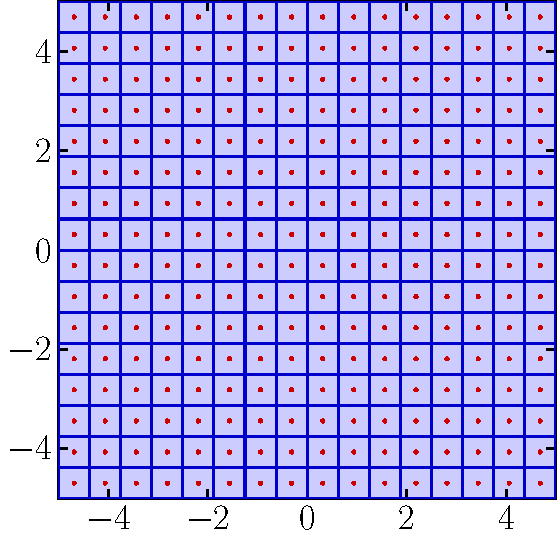
\includegraphics{TrCoding/UniformScalarLloyd4bit_New.pdf}}
    \end{center}
  \end{minipage}%
  \begin{minipage}[t]{0.5\linewidth}
    \begin{center}
      {\bf~LBG} ($N=2$): \;SNR\,=\,24.14\,dB\\[1ex]
      \hfitbox{0.6\linewidth}{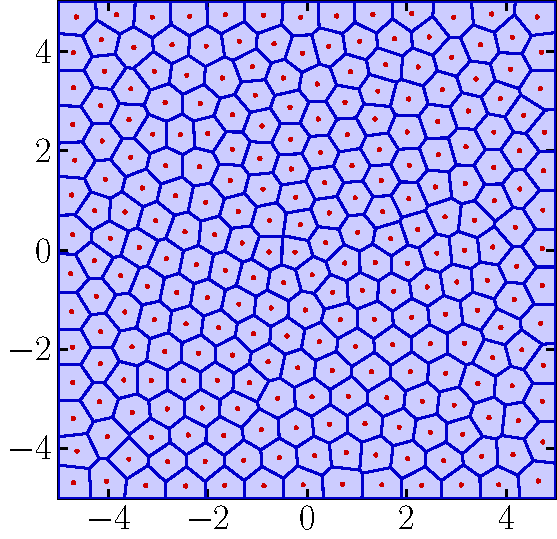
\includegraphics{TrCoding/UniformLloyd4bit_final_New.pdf}}
    \end{center}
  \end{minipage}

  \bit
\item\medskip LBG algorithm approaches approximate hexagonal lattice
\item[\iarrow]\smallskip Improvement of 0.17\,dB
  \eit
\end{frame}



\begin{frame}{Shape and memory advantage}
\bit
\item Given an $\mathbb{R}^N$-valued source $X=(X_1,\dots,X_N)$ with distribution $p_X$. 
\item Let $p_{X_i}$ denote the marginal distribution of the $i$-th component $X_i$ with  density $\tilde{f}$.  
\item Assume $X$ is stationary, in particular, marginal probabilities satisfy $p_{X_i}=p_{X_j}$ for all $i, j$. 
\item \loud{Shape and memory advantage: } Compare source-dependent terms in Panter and Dite formula for 1-dimensional and $N$-dimensional case invoking density $f$ and 
density $\tilde{f}$.
\eit 
\vspace{-0.1em}
Shape and memory advantage depend on source $X$. \loud{\iarrow$ $ Idea of transform coding: }
\bit
\item Modify source $X$, code $\phi(X)$ instead of $X$ . Use scalar quantizers for $\phi(X)$. 
\item A priori, $\phi$ can be \textit{any} deterministic mapping that is invertible with inverse $\phi^{-1}$. 
\item Distribution of  individual components of $\phi(X)$ is different than for $X$.
\item Design goal: Reduce impact of shape and memory advantage for $\phi(X)$ compared to original $X$.
\item More informally: Try to achieve \loud{energy compaction} by concentrating main information contained in $\phi(X)$ in its first few components.
\item \ALERT{Transform coding}: Mapping $\phi$ is linear, $\phi$ is a \loud{transform}.   
\eit
\end{frame}





\section{The Karhuenen Loewe Transform} 
\begin{frame}
 \vspace{12.0ex}
\begin{center}
\begin{beamercolorbox}[sep=12pt,center]{part title}
\usebeamerfont{section title}\insertsection\par
\end{beamercolorbox}
\end{center}
\end{frame}

\begin{frame}\frametitle{Low rank approximation}

\loud{Goal of low rank approximation: }
\bit
\item Try to represent $X$ in a different coordinate system such that first components carry most meaningful information on $X$. 
\item[\iarrow]  For each $k\in\{1,\dots,N\}$, find \loud{best $k$-dimensional approximation of $X$.}
\eit
\loud{Formal definition:} 
\bit  
\item For each $k$, find $k$-dimensional subspace $V$ of $\mathbb{R}^N$ which is of minimal expected distance 
to $X$, i.e. which solves
\begin{align}\label{BestApproxMin}
\underset{V\colon \dimension(V)=k}{\min}\mathbb{E}(\dist(V,X)^2).
\end{align} 
\item Here, $\dist$ denotes the Euclidean distance:
\begin{align*}
dist(x,V)=\min_{v\in V}\left\|x-v\right\|, \quad x\in\mathbb{R}^N. 
\end{align*} 
\item Minimum in \eqref{BestApproxMin} is taken over all $k$-dimensional subspaces of $\mathbb{R}^N$.
\eit
\end{frame}


\begin{frame}\frametitle{Energy compaction}
\begin{itemize}
\item If $V$ is a $k$-dimensional subspace of $\mathbb{R}^N$, let $v_1,\dots,v_N$ be an orthonormal basis of $\mathbb{R}^N$ such 
that $v_1,\dots,v_k$ is an orthonormal basis of $V$. Then:
\begin{align}\label{normminusdist}
\mathbb{E}(\dist(V,X)^2)=&\sum_{i=k+1}^N\mathbb{E}\left(<X,v_i>^2\right)\nonumber\\
=&\mathbb{E}(\left\|X\right\|^2)-\sum_{i=1}^k\mathbb{E}\left(<X,v_i>^2\right).
\end{align}
\item By \eqref{normminusdist}, $V$ minimizes \eqref{BestApproxMin} if and only if each orthonormal basis $v_1,\dots,v_k$ of $V$ solves
\begin{align}\label{BestApproxMax}
\underset{\underset{<v_i,v_j>=\delta_{i,j} \colon \forall i,j\in\{1,\dots,k\}}{\{v_1,\dots,v_k\}}}{\max}\mathbb{E}(<X,v_1>^2)+\dots+\mathbb{E}(<X,v_k>^2).
\end{align} 
Here $\delta_{i,j}=1$ if $i=j$ and $\delta_{i,j}=0$, else.
\item An orthonomal set which solves \eqref{BestApproxMax} \loud{optimally concentrates or compacts the energy of $X$ in $k$ components}. 
\item[\iarrow] \loud{Low rank approximation and energy compaction are equivalent problems.}
\end{itemize}
\end{frame}


\begin{frame}\frametitle{Autocorrelation matrix} 
\loud{How does one achieve energy compaction:} 
\bit
\item Assume from now that $X$ is of \loud{zero mean}. 
\item The matrix 
\begin{align*}
R_X:=\mathbb{E}(XX^t)
\end{align*}
is called \loud{autocorrelation matrix }of $X$.
\eit

\loud{Properties of the autorcorrelation matrix $R_X$:}
\bit
\item The $i$-th diagonal element $R_X(i,i)$ of $R_X$ is the variance $\sigma_i^2(X)$
of $X_i$. 
\item $R_X$ is symmetric.
\item For any $v\in\mathbb{R}^N$ one has 
\begin{align*}
v^tR_Xv=\mathbb{E}(<v,X>^2)\geq 0.
\end{align*}
In particular, $R_X$ is positive semidefinite. 
\item For an $N\times N$-Matrix $T$, one has 
\begin{align*}
R_{TX}=TR_XT^t. 
\end{align*}
\eit
\end{frame}

\begin{frame} \frametitle{The Karhuenen Loeve Transform (KLT)}
\loud{Definition of a KLT:}
\bit
\item An orthogonal matrix $T$ for which 
$R_{TX}=TR_{X}T^t$ is a diagonal matrix is called a KLT for $X$. 
\item Since $R_X$ is symmetric, it is diagonalizable and there exists an orthonormal basis of eigenvectors. 
\item [\iarrow] A KLT always exists.
\eit
\loud{Basic properties of KLTs:}
\bit 
\item The rows of the KLT comprise an orthonormal basis of eigenvectors of $R_X$. 
\item If the eigenvalues of $R_X$ are all distinct, a KLT is unique up to permutations and multiplications by $\pm 1$ of its rows. 
\item No general algorithm to exactly compute the eigenvalues of $R_X$ exists.
\item Well working iterative schemes for compuation of KLT which are convergent:
\bit 
\item QR-method 
\item Jacobi method
\eit
\eit
\end{frame}

\begin{frame}\frametitle{KLT yields optimal energy compaction}
\begin{proposition}[Optimal Energy Compaction of the KLT]\label{TheoremKLTEnergy}
Let $\lambda_1,\dots,\lambda_N$ denote the eigenvalues of $R_X$, ordered such that 
\begin{align*}
\lambda_1\geq \lambda_2\geq\dots\geq \lambda_N\geq 0
\end{align*}
and let be $\{v_1,\dots,v_N\}$ be an associated orthonormal basis of eigenvectors.
\bit
\item For every $k\in\{1,\dots,N\}$, the set $\{v_1,\dots,v_k\}$ solves  \eqref{BestApproxMax}. 
\item Equivalently, for 
every $k\in\{1,\dots,N\}$, the space 
\begin{align*}
V_k:=\mathbb{R}v_1\oplus\cdots\oplus\mathbb{R}v_k
\end{align*}
solves \eqref{BestApproxMin}.
\eit
\end{proposition}
\loud{\iarrow For a given source $X$, KLT computs best low-rank approximation of $X$.}
\end{frame}

\begin{frame}\frametitle{Proof of optimal energy compaction of KLT for $k=1$.}
\begin{itemize}
\item For $k=1$, one needs to finde $v_1\in\mathbb{R}^N$ which solves the constraint optimization problem 
\begin{align}\label{maximization}
 & \text{maximize}\quad &\mathbb{E}(<X,v>^2) \nonumber \\ & \text{subject to}\quad &\left\|v\right\|^2=1.
\end{align}
\item One has 
\begin{align}\label{ExpValSP}
\mathbb{E}(<X,v>^2)=\mathbb{E}(v^tXX^tv)
=v^tR_Xv.
\end{align}
\item By the Lagrangian multiplier law, $v_1$ satisfies  
\begin{align*}
&\gradient\mathbb{E}(<X,v_1>^2) =\lambda \gradient\left\|v_1\right\|^2 
\iff &2R_Xv_1=2\lambda v_1
\end{align*}
for some $\lambda\in\mathbb{R}$. 
\item Thus, $v_1$ needs to be an eigenvector of $R_X$ of eigenvalue $\lambda$. By \eqref{ExpValSP}, one 
has 
\begin{align*}
\mathbb{E}(<X,v>^2)=\lambda^2
\end{align*}
and thus \eqref{maximization} is maximized if $\lambda=\lambda_1$. 
\end{itemize}
\end{frame}

\begin{frame}\frametitle{Proof of optimal energy compaction of KLT  for general $k$, I }
\begin{itemize}
\item Perform induction on k. Assume that the statement holds for $v_1,\dots,v_{k-1}$. 

\item Let $v_k$ be a solution of the constraint optimization problem 
\begin{align}\label{maximizationGen}
 & \text{maximize} &\mathbb{E}(<X,v>^2) \nonumber \\ & \text{subject to}\: &\left\|v\right\|^2=1\: \text{and}<v,v_i>=0, \:\forall i\in\{1,\dots,k-1\}.
\end{align}
\item Again, by the Lagrangian multiplier law there exist $\lambda,\:\mu_1,\dots,\mu_{k-1}\in\mathbb{R}$ such that
\begin{align*}
2R_Xv_k=2\lambda v_k+\mu_1v_1+\dots+\mu_{k-1}v_{k-1}. 
\end{align*}
\item Since $R_Xv_i=\lambda_i$, taking the scalar product with $v_i$ implies 
\begin{align*}
0=2\lambda_iv_i^tv_k=(2R_Xv_i)^tv_k=2v_i^tR_Xv_k=\mu_i.
\end{align*}
for each $i\in\{1,\dots,k-1\}$. 
\item Thus $v_k$ is an eigenvector of $R_X$ with eigenvalue $\lambda$. Maximizing \eqref{maximizationGen} implies 
$\lambda=\lambda_k$. 
\end{itemize}
\end{frame}

\begin{frame}\frametitle{Proof of optimal energy compaction of KLT  for general $k$, II}
\begin{itemize}
\item Let $W$ be an arbitrary $k$-dimensional subspace of $\mathbb{R}^N$. Then $W$ contains a vector $w$ which is orthogonal to $v_1,\dots,v_{k-1}$. 
\item Choose vectors $w_1,\dots,w_{k-1}$ such that $\{w_1,\dots,w_{k-1},w\}$ is an orthonormal basis of $W$. 
\item By induction hypothesis and 
by the property of $v_k$ one has 
\begin{align*}
&\sum_{i=1}^{k-1}\mathbb{E}(<X,w_i>^2)+\mathbb{E}(<X,w>^2)\\
\leq& \sum_{i=1}^{k-1}\mathbb{E}(<X,v_i>^2)+\mathbb{E}(<X,v_k>^2). 
\end{align*}
\item By \eqref{normminusdist}, this implies
\begin{align*}
\mathbb{E}(\dist(X,W)^2)\geq \mathbb{E}(\dist(X,V_k)^2).
\end{align*}
\end{itemize}
\qed
\end{frame}

\section{Principal Component Analysis}

\begin{frame}
 \vspace{12.0ex}
\begin{center}
\begin{beamercolorbox}[sep=12pt,center]{part title}
\usebeamerfont{section title}\insertsection\par
\end{beamercolorbox}
\end{center}
\end{frame}




\begin{frame}\frametitle{KLT and Principal Component Analysis}
\loud{Definition of principal component analysis} 
\begin{itemize}
\item Let $\lambda_1\geq\dots\geq \lambda_N$ be the eigenvalues of $R_X$ and let $T$ be a KLT for $X$. 
\item Reorder 
rows of $T$ such that $i$-th row is an eigenvector of $T$ of eigenvalue $\lambda_i$.
\item The $i$-th row of $T$ is called the i-th \loud{principal component} of $X$. 
\item Consider the random variable 
\begin{align*}
Y=TX=\begin{pmatrix}Y_1\\ \vdots\\Y_N\end{pmatrix}
\end{align*}
instead of $X$
\item First few components of $Y$ carry the most meaningful information 
about $X$.  
\item Given a realization $x\in\mathbb{R}^N$ of $X$, computing the first $k$ components $y_1,\dots,y_k$ of $Tx$,
where often $k\ll N$,  is called principal component analysis (PCA). 
\end{itemize}
\end{frame}


\begin{frame}\frametitle{PCA for analysis of large data sets}
\begin{itemize}
\item Random variable $X$ is often derived as an empirical distribution.
\item Assume that $d$ measurements $x_d\in\mathbb{R}^N$ of $N$ variables are conducted where typically $d\gg N$. 
Let $x_{i,j}$ be the value of the $j$-th variable at the $i$-th measurement. 
For $j\in\{1,\dots,N\}$ let 
\begin{align*}
\mu_j:=\frac{1}{d}\sum_{i=1}^dx_{i,j}
\end{align*}
denote the $j$-th empirical mean and let $\overline{x}_{i,j}:=x_{i,j}-\mu_j$ be the 
mean-corrected measurements. 
\item Then the $d\times N$ matrix whose 
$i$-th row and $j$-th column is given by $\overline{x}_{i,j}$ is often called (normalized) data matrix $M_{data}$.
\item The auto-covariance matrix of the empirical distribution $X$ defined by the $\overline{x}_{i,j}$ is 
given by 
\begin{align*}
R_X=M_{data}^tM_{data}. 
\end{align*}
\end{itemize}
\end{frame}

\begin{frame}\frametitle{Example of a PCA}
Taken from Bishop, Pattern Recognition and Machine Learning 
\begin{itemize}
\item Consider a dataset that consists of a large collection of handwritten digits of the number $3$, taken from MNIST dataset.
\item Each data-sample of an handwritten digit is a grey-scale image with $28\times 28$ pixels. 
\item Thus: Data samples correspond to vectors $x_d\in \mathbb {R}^N$ for $N=748$. 
\end{itemize}
\begin{figure}
\centering
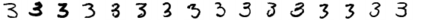
\includegraphics[width=0.95\textwidth]{TrCoding/number_3_MNIST.png}
\captionsetup{labelformat=empty}
\caption{Example for handwritten digits from MNIST.}
\end{figure}
\end{frame}

\begin{frame}{ Visualization of principal components} 
\begin{itemize}
\item PCA: Let $\lambda_1\geq\lambda_2\geq\cdots\geq \lambda_N$ denote the eigenvalues 
of the empirical covariance matrix, and $v_1,\dots,v_N$ be the assiocated eigenvectors, the principal components.
\end{itemize}
\begin{figure}
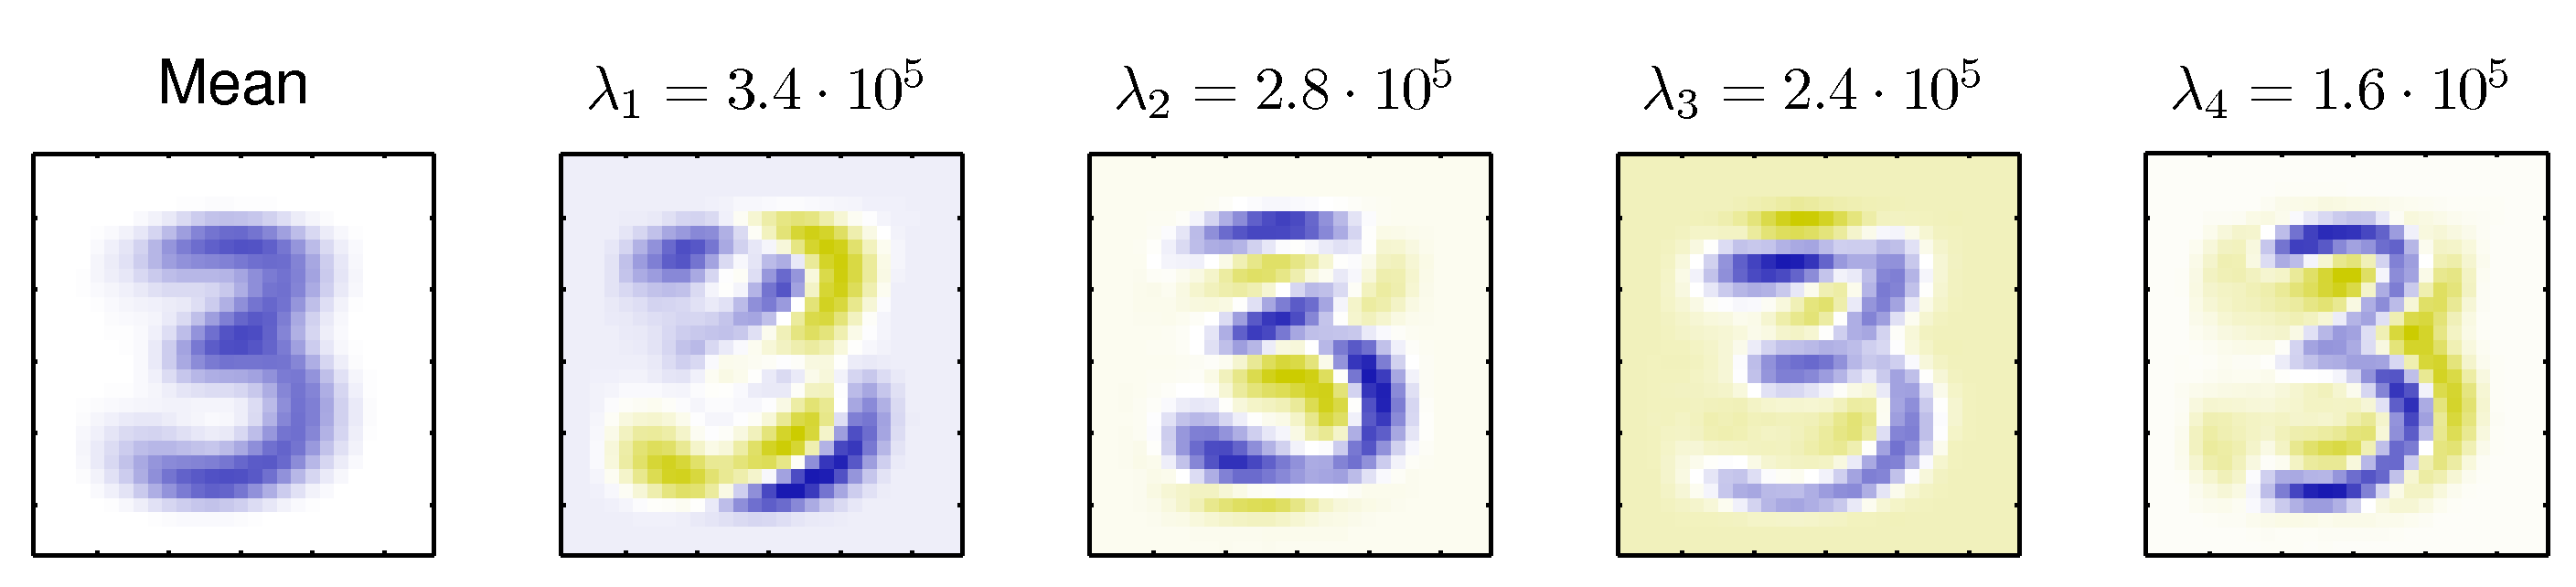
\includegraphics[width=0.5\textwidth]{TrCoding/FigurePCA_1.png}
\captionsetup{labelformat=empty}
\caption{The mean (blue) and the first four principal components $v_1,\dots,v_4$ (yellow) of the handwritten digits of the number 3. }
\end{figure}
\end{frame}

\begin{frame}{Visualization of energy compaction of PCA}
\begin{figure}
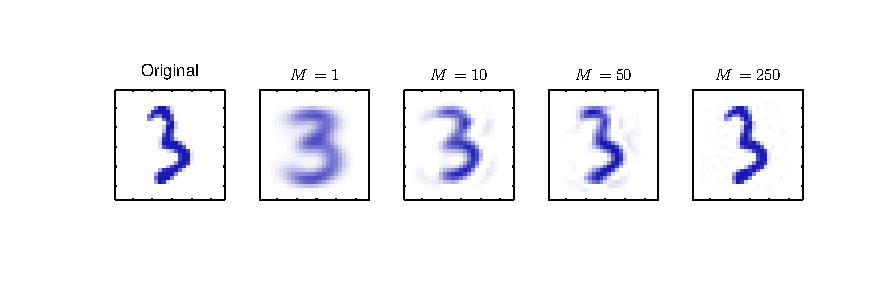
\includegraphics[width=0.75\textwidth]{TrCoding/FigurePCAEx.pdf}
\captionsetup{labelformat=empty}
\caption{Original handwritten digit (left), and its representation by using only a subset $v_1,\dots,v_M$ of the principal components. If $x\in\mathbb{R}^{748}$, the $M$-th picture 
represents
  \begin{minipage}{\linewidth}
     \begin{equation*}
        \mu+\sum_{i=1}^M<x,v_i>v_i,
   \end{equation*}
   \end{minipage}
where $\mu\in\mathbb{R}^N$ is the mean of the data. 
}
\end{figure}
\end{frame} 


\section{Definition of transform coding}


\begin{frame}
 \vspace{12.0ex}
\begin{center}
\begin{beamercolorbox}[sep=12pt,center]{part title}
\usebeamerfont{section title}\insertsection\par
\end{beamercolorbox}
\end{center}
\end{frame}

\begin{frame}\frametitle{Transform coding}

\begin{definition}[Transform coding]
Let $S$ be an $N$-dimensional source. Invertible $N\times N$-matrices $A, B$ and scalar quantizers $Q_1,\dots,Q_N$ 
define the transform coding of $s\in\mathbb{R}^N$ , realization of $S$, as the following ordered steps:
\begin{enumerate}
\item Compute $u=As$. The components $u_1,\dots,u_N$ of $u$ are called transform coeffients. 
\item Code each $u_i$ with $Q_i$ to obtain the reconstructed transform coefficients $u_i'$ which comprise the reconstructed transformed vector $u'$. 
\item Compute the reconstructed vector $s'$ as $s'=Bu'$.   
\end{enumerate}
\end{definition}
\bit
\item The matrix $A$ is called \loud{analysis transform}.
\item The matrix $B$ is called \loud{synthesis transform}. 
\item In most cases, one has $B=A^{-1}$. 
\eit
\end{frame}



\begin{frame}{Structure of Transform Coding Systems}
  \vspace{-2ex}
\begin{center}
  \hfitbox{0.70\linewidth}{%
  \begin{tikzpicture}
     [
      pstep/.style={
        draw=black,
        fill=white,
        line width=0.75pt,
        minimum width=1.2cm,
        minimum height=0.7cm,
        inner sep=0,
        align=center
      },
      nbox/.style={pstep,
        rectangle
      },
      tbox/.style={nbox,
        draw=blue,text=blue,fill=blue!10,
        line width=1.0pt,
        minimum width=1.8cm,
        minimum height=5.0cm
      },
      narrow/.style={
        line width=0.75pt,
        -{Latex[length=2.5mm,width=1.4mm]}
        },
    ]
    \node[nbox] (q0) at ( 0.00, 0.00) {\relsize{2}$Q_0$};
    \node[nbox] (q1) at ( 0.00,-1.00) {\relsize{2}$Q_1$};
    \node[nbox] (q2) at ( 0.00,-2.00) {\relsize{2}$Q_2$};
    \node[]          at ( 0.00,-2.90) {\relsize{2}$\vdots$};
    \node[nbox] (qx) at ( 0.00,-4.00) {\relsize{2}$Q_{N-1}$};
    \node[tbox] (a)  at (-3.30,-2.00) {\relsize{3}$\ve{A}$};
    \node[tbox] (b)  at ( 3.30,-2.00) {\relsize{3}$\ve{B}$};
    \draw[narrow] (a.east |- q0.east) -- (q0) 
          node[pos=0.50,anchor=base,yshift=1.3ex] {\relsize{2}$u_0$};
    \draw[narrow] (a.east |- q1.east) -- (q1) 
          node[pos=0.50,anchor=base,yshift=1.3ex] {\relsize{2}$u_1$};
    \draw[narrow] (a.east |- q2.east) -- (q2) 
          node[pos=0.50,anchor=base,yshift=1.3ex] {\relsize{2}$u_2$};
    \draw[narrow] (a.east |- qx.east) -- (qx) 
          node[pos=0.50,anchor=base,yshift=1.3ex] {\relsize{2}$u_{N-1}$};
    \draw[narrow] (q0) -- (q0.west -| b.west) 
          node[pos=0.50,anchor=base,yshift=1.3ex] {\relsize{2}$u'_0$};
    \draw[narrow] (q1) -- (q1.west -| b.west) 
          node[pos=0.50,anchor=base,yshift=1.3ex] {\relsize{2}$u'_1$};
    \draw[narrow] (q2) -- (q2.west -| b.west) 
          node[pos=0.50,anchor=base,yshift=1.3ex] {\relsize{2}$u'_2$};
    \draw[narrow] (qx) -- (qx.west -| b.west) 
          node[pos=0.50,anchor=base,yshift=1.3ex] {\relsize{2}$u'_{N-1}$};
    \node[] (in) at (-6.5,-2.0) 
         {\relsize{2}$\displaystyle\left[\!\!\begin{array}{c}
           s_0\\[.2ex]s_1\\[.2ex]s_2\\[.2ex]\vdots\\[.2ex]s_{N-1}\\[.5ex]
          \end{array}\!\!\right]$};
    \node[] (out) at (6.5,-2.0) 
         {\relsize{2}$\displaystyle\left[\!\!\begin{array}{c}
           s'_0\\[.2ex]s'_1\\[.2ex]s'_2\\[.2ex]\vdots\\[.2ex]s'_{N-1}\\[.5ex]
          \end{array}\!\!\right]$};
    \draw[narrow] (in) -- (a);
    \draw[narrow] (b)  -- (out);
    \node[anchor=north east,align=right,text=blue,yshift=-0.5ex] 
          at (a.south east) {\relsize{2}analysis\\[.2ex]\relsize{2}transform};
    \node[anchor=north west,align=left,text=blue,yshift=-0.5ex] 
          at (b.south west) {\relsize{2}synthesis\\[.2ex]\relsize{2}transform};
    \node[anchor=north,align=center,yshift=-1.8ex] 
          at (qx.south) {\relsize{2}scalar\\[.2ex]\relsize{2}quantizers};
  \end{tikzpicture}
  }
\end{center}

\bold{Effect of transform coding}:
\bit
\item Remove/reduce dependencies before scalar quantization
\item Simple alternative to vector quantization
\item Simple and most relevant case: Linear transforms
\eit
\end{frame}



\begin{frame}{Transform Encoder and Transform Decoder}
\vspace{-2ex}
\begin{center}
  \hfitbox{0.75\linewidth}{%
  \begin{tikzpicture}
     [
      pstep/.style={
        draw=black,
        fill=white,
        line width=0.75pt,
        minimum width=1.2cm,
        minimum height=0.7cm,
        inner sep=0,
        align=center
      },
      nbox/.style={pstep,
        rectangle
      },
      sbox/.style={nbox,myred,fill=myred!10,text=myred},
      tbox/.style={nbox,
        minimum width=2.2cm,
        minimum height=3.1cm
      },
      narrow/.style={
        line width=0.75pt,
        -{Latex[length=2.5mm,width=1.3mm]}
        },
    ]
    \draw[fill=gray!10,draw=none] (-5.0,2.3) rectangle (5.0,-1.8);
    \node[anchor=north west,xshift=0.5ex,yshift=-0.5ex,text=black!70] 
                     at (-5.00, 2.30) {\relsize{1}\ital{encoder}};
    \node[sbox] (q0) at ( 0.00, 1.20) {\relsize{2}$\alpha_0$};
    \node[sbox] (q1) at ( 0.00, 0.20) {\relsize{2}$\alpha_1$};
    \node[]          at ( 0.00,-0.40) {\relsize{2}$\vdots$};
    \node[sbox] (qx) at ( 0.00,-1.20) {\relsize{2}$\alpha_{N-1}$};
    \node[tbox,myblue,fill=myblue!10,text=myblue,align=center] (a)  at (-3.30, 0.00) 
       {
         \relsize{1}analysis\\[1ex]
         \relsize{1}transform\\[3ex]
         \relsize{2}$\ve{A}$
       };
    \node[tbox,mygreen,fill=mygreen!10,text=mygreen,align=center] (b)  at ( 3.30, 0.00) 
       {
         \relsize{1}entropy\\[1ex]
         \relsize{1}coding\\[3ex]
         \relsize{2}$\gamma$
       };
    \draw[narrow] (a.east |- q0.east) -- (q0) 
          node[pos=0.50,anchor=base,yshift=1.3ex] {\relsize{1}$u_0$};
    \draw[narrow] (a.east |- q1.east) -- (q1) 
          node[pos=0.50,anchor=base,yshift=1.3ex] {\relsize{1}$u_1$};
    \draw[narrow] (a.east |- qx.east) -- (qx) 
          node[pos=0.50,anchor=base,yshift=1.3ex] {\relsize{1}$u_{N-1}$};
    \draw[narrow] (q0) -- (q0.west -| b.west) 
          node[pos=0.50,anchor=base,yshift=1.3ex] {\relsize{1}$q_0$};
    \draw[narrow] (q1) -- (q1.west -| b.west) 
          node[pos=0.50,anchor=base,yshift=1.3ex] {\relsize{1}$q_1$};
    \draw[narrow] (qx) -- (qx.west -| b.west) 
          node[pos=0.50,anchor=base,yshift=1.3ex] {\relsize{1}$q_{N-1}$};
    \draw[narrow]       (-7.0, 0.00) -- (a);
    \draw[narrow] (b) -- (7.0, 0.00);
    \node[anchor=south west,align=left,inner sep=0pt,yshift=1.5ex] at (-7,0)
      {\relsize{1}blocks of\\[1ex]\relsize{1}samples};
    \node[anchor=north west,align=left,inner sep=0pt,yshift=-2ex,xshift=2em] at (-7,0)
      {\relsize{1}$\ve{s}$};
    \node[anchor=south east,align=right,inner sep=0pt,yshift=1.5ex] at (7,0)
      {\relsize{1}bitstream};
    \node[anchor=north east,align=right,inner sep=0pt,yshift=-2ex,xshift=-2em] at (7,0)
      {\relsize{1}$\ve{b}$};
  \end{tikzpicture}
  }

  \smallskip
  \uncover<2->{\hfitbox{0.75\linewidth}{%
  \begin{tikzpicture}
     [
      pstep/.style={
        draw=black,
        fill=white,
        line width=0.75pt,
        minimum width=1.2cm,
        minimum height=0.7cm,
        inner sep=0,
        align=center
      },
      nbox/.style={pstep,
        rectangle
      },
      sbox/.style={nbox,myred,fill=myred!10,text=myred},
      tbox/.style={nbox,
        minimum width=2.2cm,
        minimum height=3.1cm
      },
      narrow/.style={
        line width=0.75pt,
        -{Latex[length=2.5mm,width=1.3mm]}
        },
    ]
    \draw[fill=gray!10,draw=none] (-5.0,2.3) rectangle (5.0,-1.8);
    \node[anchor=north west,xshift=0.5ex,yshift=-0.5ex,text=black!70] 
                     at (-5.00, 2.30) {\relsize{1}\ital{decoder}};
    \node[sbox] (q0) at ( 0.00, 1.20) {\relsize{2}$\beta_0$};
    \node[sbox] (q1) at ( 0.00, 0.20) {\relsize{2}$\beta_1$};
    \node[]          at ( 0.00,-0.40) {\relsize{2}$\vdots$};
    \node[sbox] (qx) at ( 0.00,-1.20) {\relsize{2}$\beta_{N-1}$};
    \node[tbox,mygreen,fill=mygreen!10,text=mygreen,align=center] (a)  at (-3.30, 0.00) 
       {
         \relsize{1}entropy\\[1ex]
         \relsize{1}decoding\\[3ex]
         \relsize{2}$\gamma^{-1}$
       };
    \node[tbox,myblue,fill=myblue!10,text=myblue,align=center] (b)  at ( 3.30, 0.00) 
       {
         \relsize{1}synthesis\\[1ex]
         \relsize{1}transform\\[3ex]
         \relsize{2}$\ve{B}$
       };
    \draw[narrow] (a.east |- q0.east) -- (q0) 
          node[pos=0.50,anchor=base,yshift=1.3ex] {\relsize{1}$q_0$};
    \draw[narrow] (a.east |- q1.east) -- (q1) 
          node[pos=0.50,anchor=base,yshift=1.3ex] {\relsize{1}$q_1$};
    \draw[narrow] (a.east |- qx.east) -- (qx) 
          node[pos=0.50,anchor=base,yshift=1.3ex] {\relsize{1}$q_{N-1}$};
    \draw[narrow] (q0) -- (q0.west -| b.west) 
          node[pos=0.50,anchor=base,yshift=1.3ex] {\relsize{1}$u'_0$};
    \draw[narrow] (q1) -- (q1.west -| b.west) 
          node[pos=0.50,anchor=base,yshift=1.3ex] {\relsize{1}$u'_1$};
    \draw[narrow] (qx) -- (qx.west -| b.west) 
          node[pos=0.50,anchor=base,yshift=1.3ex] {\relsize{1}$u'_{N-1}$};
    \draw[narrow]       (-7.0, 0.00) -- (a);
    \draw[narrow] (b) -- (7.0, 0.00);
    \node[anchor=south west,align=left,inner sep=0pt,yshift=1.5ex] at (-7,0)
      {\relsize{1}bitstream};
    \node[anchor=north west,align=left,inner sep=0pt,yshift=-2ex,xshift=2em] at (-7,0)
      {\relsize{1}$\ve{b}$};
    \node[anchor=south east,align=right,inner sep=0pt,yshift=1.5ex] at (7,0)
      {\relsize{1}blocks of\\[1ex]\relsize{1}reconstr.\\[1ex]\relsize{1}samples};
    \node[anchor=north east,align=right,inner sep=0pt,yshift=-2ex,xshift=-2em] at (7,0)
      {\relsize{1}$\ve{s'}$};
  \end{tikzpicture}
  }}
\end{center}\vspace{-1ex}
\end{frame}

\end{document}
